% 
% ======================================================================
\RequirePackage{docswitch}
% \flag is set by the user, through the makefile:
%    make note
%    make apj
% etc.
\setjournal{\flag}

\documentclass[\docopts]{\docclass}

% You could also define the document class directly
%\documentclass[]{emulateapj}

% Custom commands from LSST DESC, see texmf/styles/lsstdesc_macros.sty
\usepackage{lsstdesc_macros}

\usepackage{graphicx}
\graphicspath{{./}{./figures/}}
\bibliographystyle{apj}
\usepackage{subfigure}

% Add your own macros here:



% 
% ======================================================================

\begin{document}

\title{ On the cadence of the LSST SN survey(s) }

\maketitlepre

\begin{abstract}

Design notes, metrics and forecasts for the deep and wide LSST SN surveys.

\end{abstract}

% Keywords are ignored in the LSST DESC Note style:
\dockeys{latex: templates, papers: awesome}

\maketitlepost

% ----------------------------------------------------------------------
% 

\section{Introduction}
\label{sec:intro}

LSST has the capability to discover $O(10^5)$ SNe~Ia in the redshift
range $0.03 < z < 0.4$ (wide survey) and $0.3 < z < 1.1$ (DDF
survey). The question of how many of these events will have light
curves of sufficient quality to be included in a Hubble diagram
remains open.  It is essentially a function of the cadence and depth
that will be delivered by the Wide and DDF surveys.

In this note, we examine the cadence envisioned for the 10 years of
LSST operations.  We base ourselves



% This is a paper and note template for the LSST DESC
% \citep{Overview,ScienceBook,WhitePaper}.  You can delete all this
% tutorial text whenever you like.

% You can easily switch between various \LaTeX\xspace styles for
% internal notes and peer reviewed journals.  Documents can be
% compiled using the provided \code{Makefile}.  The command
% \code{make} with no arguments compiles \code{main.tex} using the
% \code{lsstdescnote.cls} style.  If you want to upgrade your Note
% into a journal article, just choose a journal name, between
% \code{make apj} (ApJ preprint format), \code{make apjl} (which uses
% the \code{emulateapj} style), \code{make prd}, \code{make prl}, and
% \code{make mnras}.


% ----------------------------------------------------------------------

\section{Design notes}
\label{sec:design_notes}

\paragraph{Redshift-limited survey} A key design quantity is the
redshift limit ($z_{lim}$) of the survey. Here, we do not refer to a
detectability limit, but to the redshift value beyond which we start
losing a fraction of the sample, because the follow-up is not good
enough (1) to measure a distance and (2) to perform a photometric
identification.  Beyond this redshift limit, one has to estimate the
fraction of events lost. This procedure yields uncertainties, that are
quite intricated with (1) the control of the demographic evolution of
SNe~Ia (2) the standardization procedures (see impact on $\beta$).  As
a consequence, the supernovae beyond $z_{lim}$ are of limited
usefulness.  Rather, we need to define, for each of our two surveys
(DDF and wide) a nominal $z_{lim}$, and aim at building a sample that
is complete up to $z_{lim}$. 

By ``complete'', we mean that, each SN~Ia occurring:
\begin{itemize}
\item in a well defined observer-frame time interval (that corresponds
  to a season) $[T_{start}; T_{end}]$;
\item in the redshift range $0.05 < z < z_{lim}$;
\item in a region of the SN~Ia parameter space that is large enough to
  encompass a potential evolution with redshift of the SN~Ia
  demographic properties;
\end{itemize}
has a follow-up which is ``good enough'' to (1) identify it
photometrically as a SN~Ia and (2) derive a standardized distance from
its lightcurve.

\paragraph{Fiducial SN~Ia parameter space region} Up to a good
approximation, SNe~Ia form a 2-dimensional family, that may be indexed
for example with color and lightcurve-width (for example, the
SALT2-color and the SALT2-$X_1$-parameter).  On figure
\ref{fig:jla_X1_C}, we show the distribution of the JLA supernovae, in
the $(X_1,C)$ parameter space. We note sizeable differences between the
nearby and distant SNe, in particular in $X_1$.  However, the full JLA
sample is well contained in the region $X_1 = [-3,3], Color= = [-0.3,
0.3]$. 

\begin{figure}[t]
\begin{center}
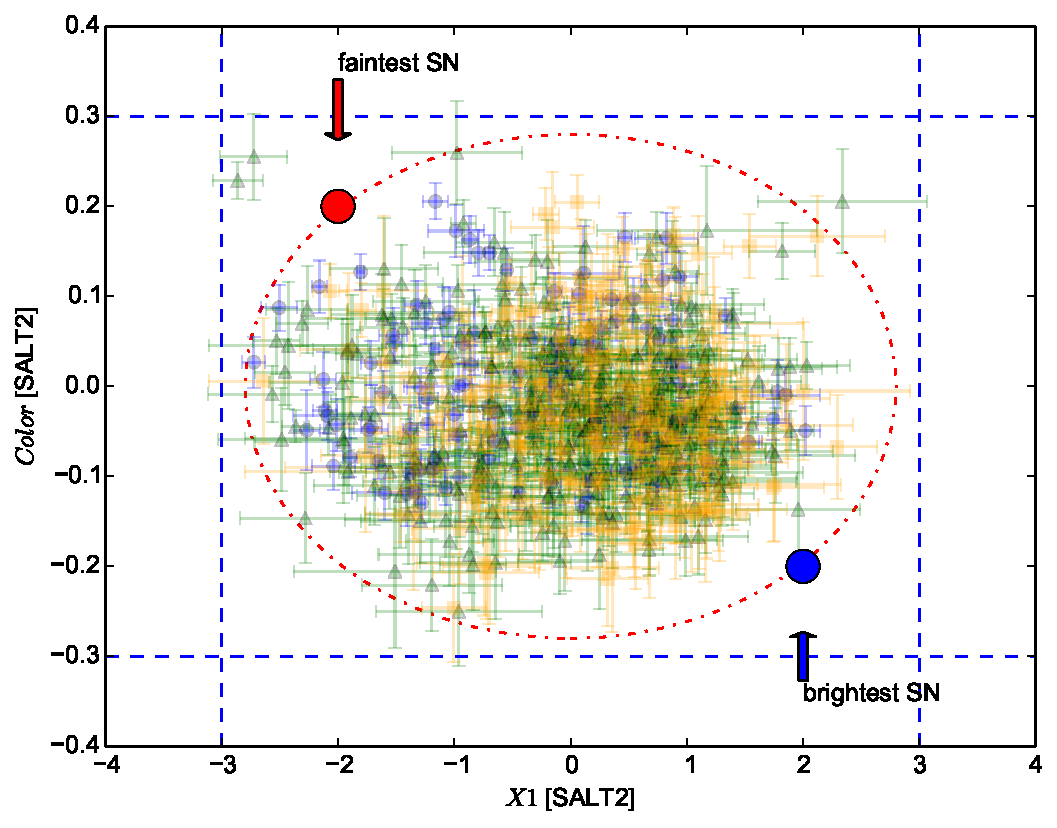
\includegraphics[width=0.75\linewidth]{sn_parameter_space.pdf}
\caption{JLA supernovae the $(X_1,Color)$ parameter space -- (blue:
  nearby, green: SDSS, orange: SNLS).  }
\label{fig:jla_X1_C}
\end{center}
\end{figure}

On the same figure, we have marked in red the faintest SN in that
parameter space ($X_1=-3, Color=0.3$). To be complete up to $z_{lim}$,
the survey has to deliver a cadence that allows to derive a luminosity
distance and a photometric identification for that event at a redshift
$z_{lim}$.

\paragraph{Lightcurve quality requirements} Our lightcurve quality
requirements are as follows:

\begin{equation}
  \mu = m^\star_B + \alpha X_1 - \beta C
\end{equation}

\begin{itemize}
\item we need measurements in at least two bands, in order to
  constrain the restframe color of the SN. Given the high intrinsic
  dispersions of SNe~Ia in the restframe UV, these bands must sample
  to the restframe region $3800 \angstrom < \lambda < 7000 \angstrom$.

\item we require the light curve shape to be well sampled in the
  (restframe) phase interval $[-10;+30]$ days, with at least four
  visits before peak (each of those visits in any of the eligible
  band), and ten visits after peak.
  
\item finally, we require that the photon noise contribution to the
  distance measurement is subdominant w.r.t. the intrinsic dispersion
  of the SNe (after standardization).  There are several ways to
  quantify this.  The dominant contribution is carried by the color
  (since $\beta \sim 3$). This means that requiring $\sigma C < 0.03$
  ensures that $\sigma \mu < 0.1$, below the intrinsic dipersion in
  the Hubble diagram, after standardization.

  Another way to look at this consists in placing requirements on the
  uncertainty of the amplitude of the lightcurve shape. 
\end{itemize}

Our goal is to make sure that the light curves of our faintest
$(X_1=-3, C=0.3)$ SNe~Ia around $z = z_{lim}$ pass these requirements.


% ----------------------------------------------------------------------

\section{A metric to evaluate a cadence}
\label{sec:methods}

\subsection{The signal-to-noise on the light-curve amplitude}

In this section, we present a metric 

If we fit a model $A \times \ell(t)$ on a lightcurve $(t_i, y_i)$, the
least square estimate of the amplitude is:
\begin{equation}
  \hat{A} = \frac{\sum_i w_i \ell_i y_i}{\sum_i w_i \ell^2_i}
\end{equation}
where we note $\ell(t_i) = \ell_i$. The  variance of $\hat{A}$ is:
\begin{equation}
  \mathrm{Var}(\hat{A}) = \left(\sum_i w_i \ell^2_i\right)^{-1}
\end{equation}
and signal to noise we get on the amplitude $\hat{A} /
\sigma_{\hat{A}}$ is:
\begin{equation}
  SNR = \left(\sum_i w_i L^2_i\right)^{1/2}
\end{equation}
where $L_i = A \times \ell_i$. Since we are dominated by the sky
background, the
\begin{equation}
  SNR = 5 \times \left(\sum_i L^2_i f^{-2}_{i|5}\right)^{1/2}
\end{equation}
This metrics is easy to compute, all it takes is a tabulated model of
the light curve shape, and a cadence file, containing, for each visit,
an assessment of the $5\sigma$-depth reached during that visit. 


\subsection{Requirements on the survey cadence and depth}

Using the metric above, we can give characterize the cadence and depth
that allow to fulfill the requirements above. 

Let's define $\delta(t_i) = \delta_i$, which is equal to the number of
observations in an interval $\Delta t$ around $t_i$. The metric above
can be rewritten:
\begin{equation}
  SNR = 5 \times \left(\sum_i \delta_i L^2_i f^{-2}_{i|5} \Delta t\right)^{1/2}
\end{equation}
where the sum runs on all the $\Delta t$ bins, in a observer frame
time interval covering the supernova lightcurve evolution. The requirement 
above can be rewritten:
\begin{equation}
  f_{|5} \left<\delta_i\right>^{-1/2} \leq \frac{5 \sqrt{\Delta t} \sqrt{\sum_i L_i^2}}{SNR}
  \label{eqn:global_metric}
\end{equation}
where $\left<\delta_i\right>$ is the cadence, weighted by the light
curve shape squared: $\left<\delta_i\right> = \sum_i \delta_i
L_i^2/\sum_i L_i^2$.  This sets a limit (in $\frac{e^-}{s}
\sqrt{day}$) on the product of the limiting flux times inverse square
root of the cadence.

This simple metric allows one to estimate the power of a cadence
without having to generate and fit supernova light curves.  Of course,
a supernova scientist is still needed, to compute the numerical values
of the upper limits that appears in equation \ref{eqn:global_metric}
For the records, we report these values in table
\ref{tab:cadence_depth_limit}. They have been computed with SALT-2.4
and the SMTN-002 instrument model.



\begin{table}[t]
\begin{center}
\caption{cadence-depth limit for the worst case SN and a target SNR=20/band}
\label{tab:cadence_depth_limit}
\begin{tabular}{l|rrrrr}
\hline
\hline
    $z$   &      $g$         &       $r$         &     $i$           &      $z$        &      $y$           \\
          &      \multicolumn{5}{c}{$[\mathrm{e^-/s \times \sqrt{day}}]$} \\
\hline
     0.4  &      86 &     267 &     279 &         &           \\
     0.5  &      31 &     153 &     148 &         &           \\
     0.6  &      12 &      81 &      94 &      92 &           \\
     0.7  &         &      42 &      69 &      57 &      34   \\
     0.8  &         &      17 &      52 &      39 &      25   \\
     0.9  &         &      11 &      32 &      31 &      17   \\
     1.1  &         &         &      11 &      20 &      11   \\
\hline
\end{tabular}
\end{center}
\end{table}



% ----------------------------------------------------------------------
\section{The DEEP LSST SN survey}

We now apply these two metrics 

\subsection{The DDF cadence from \code{Minion\_1016}}
\label{sec:results}




\begin{figure*}
\begin{center}
\subfigure[$r$]{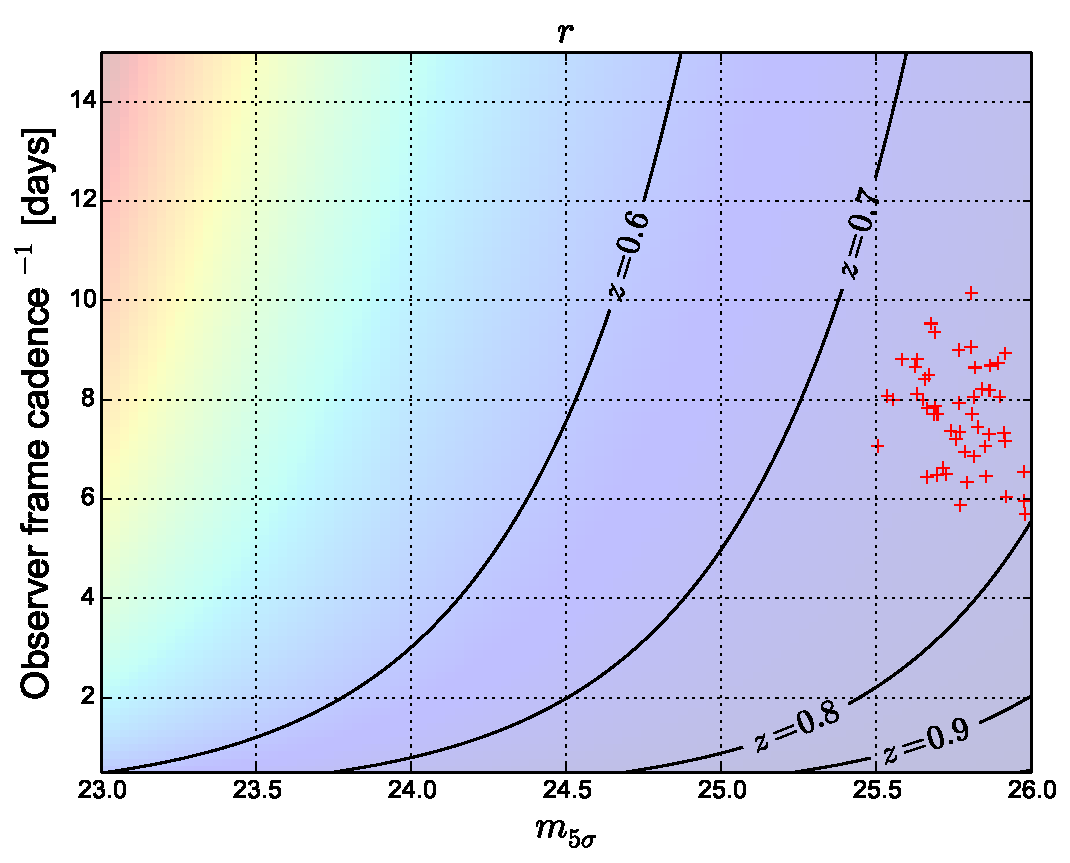
\includegraphics[width=0.48\linewidth]{m5_cadence_limits_r.pdf}}
\subfigure[$i$]{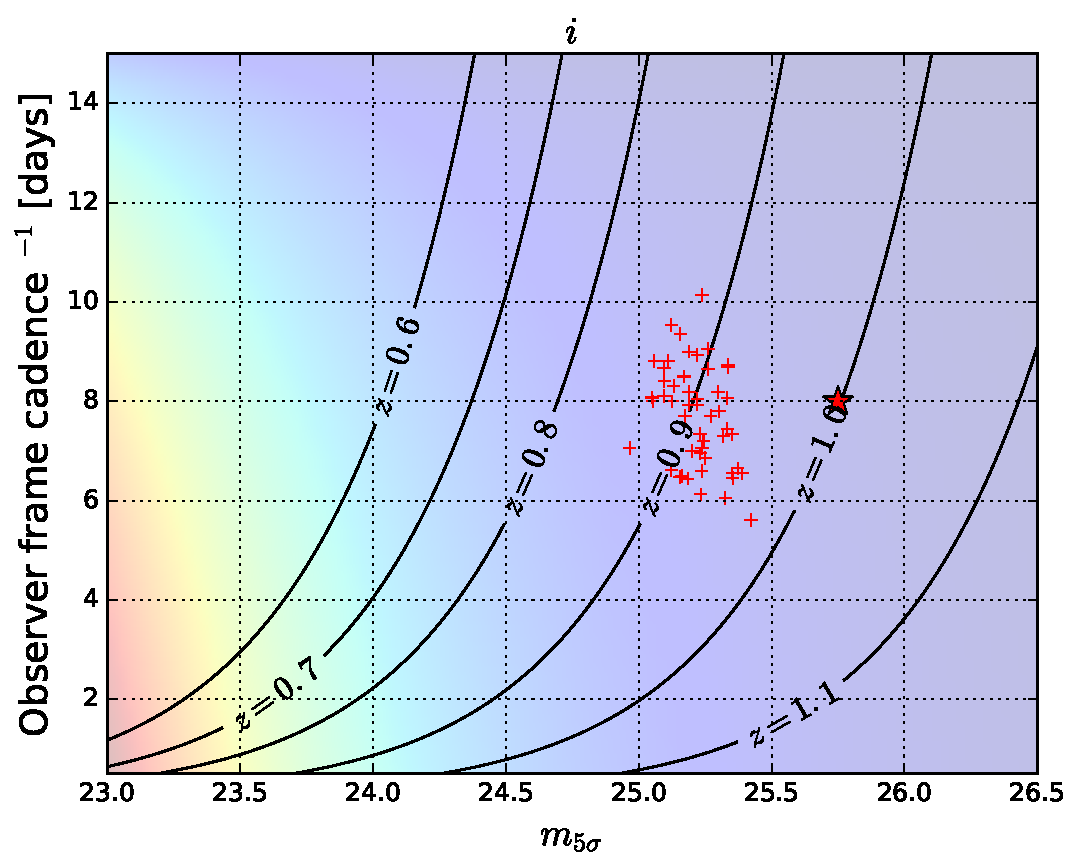
\includegraphics[width=0.48\linewidth]{m5_cadence_limits_i.pdf}}\\
\subfigure[$z$]{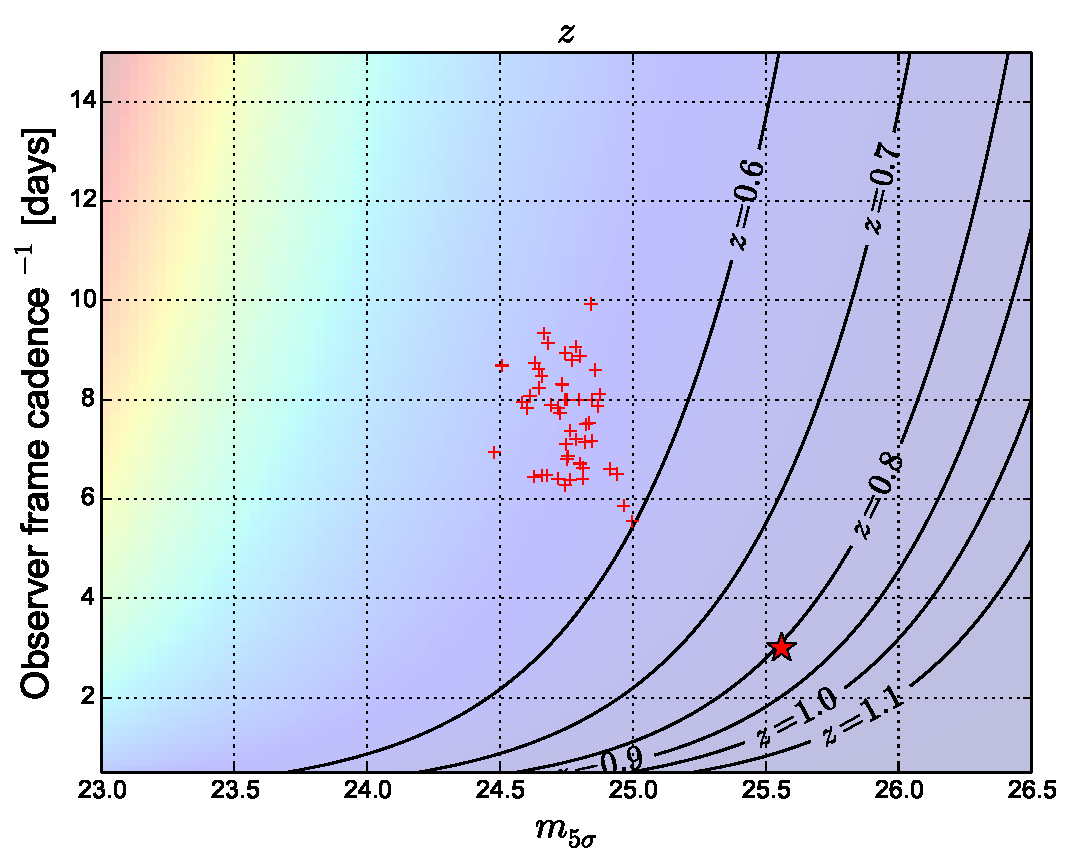
\includegraphics[width=0.48\linewidth]{m5_cadence_limits_z.pdf}}
\subfigure[$y$]{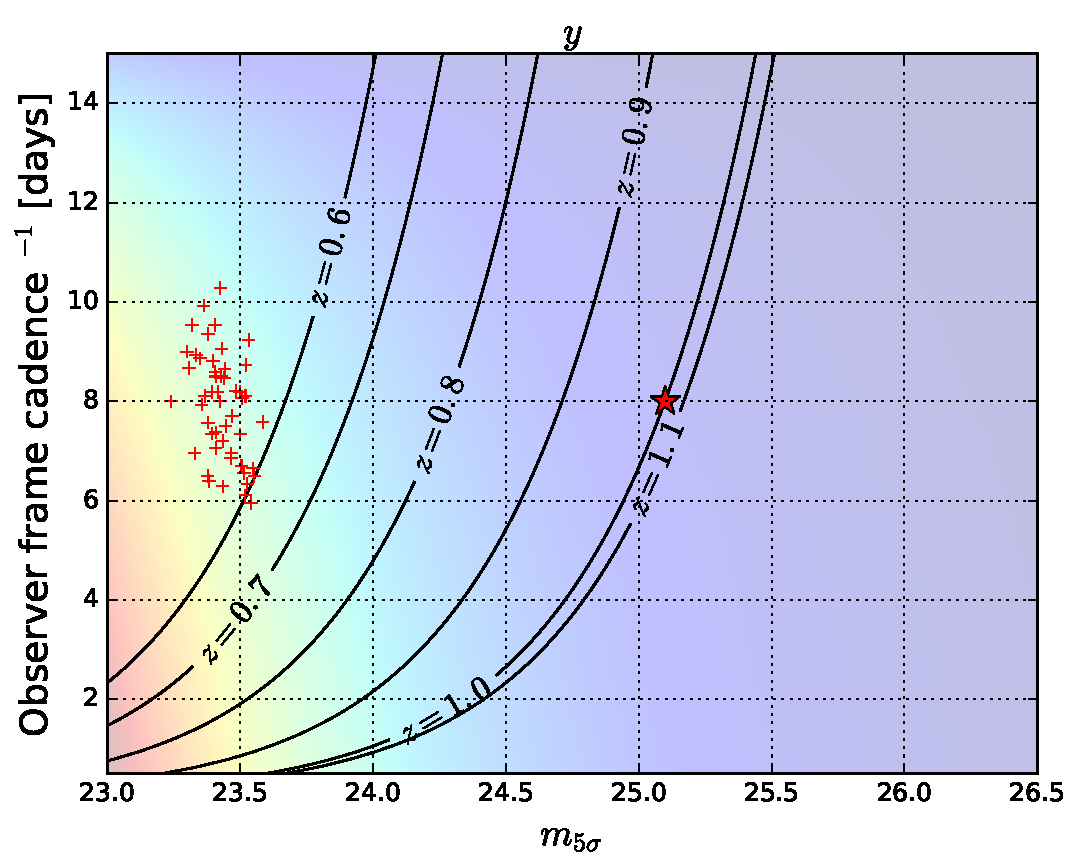
\includegraphics[width=0.48\linewidth]{m5_cadence_limits_y.pdf}}
\caption{The cadence {\em vs.} depth requirements for the DDF LSST SN
  survey in the $r,i,z$ and $y$-bands. The color scale corresponds to
  the metric described in equation \ref{eqn:global_metric}.  The lines are
  the contour-levels computed for the limits indicated on table
  \ref{tab:cadence_depth_limit}. To fulfill the SNR requirements at a
  given redshift, one has to be {\em below} the corresponding
  line. The stars indicate an ambitious -- but attainable -- goal for
  a DDF survey.  The red crosses show what the survey can currently
  deliver according to \code{Minion\_1016}. }
\label{fig:m5_cadence_limits_ddf}
\end{center}
\end{figure*}



\begin{figure*}[t]
  \begin{center}
    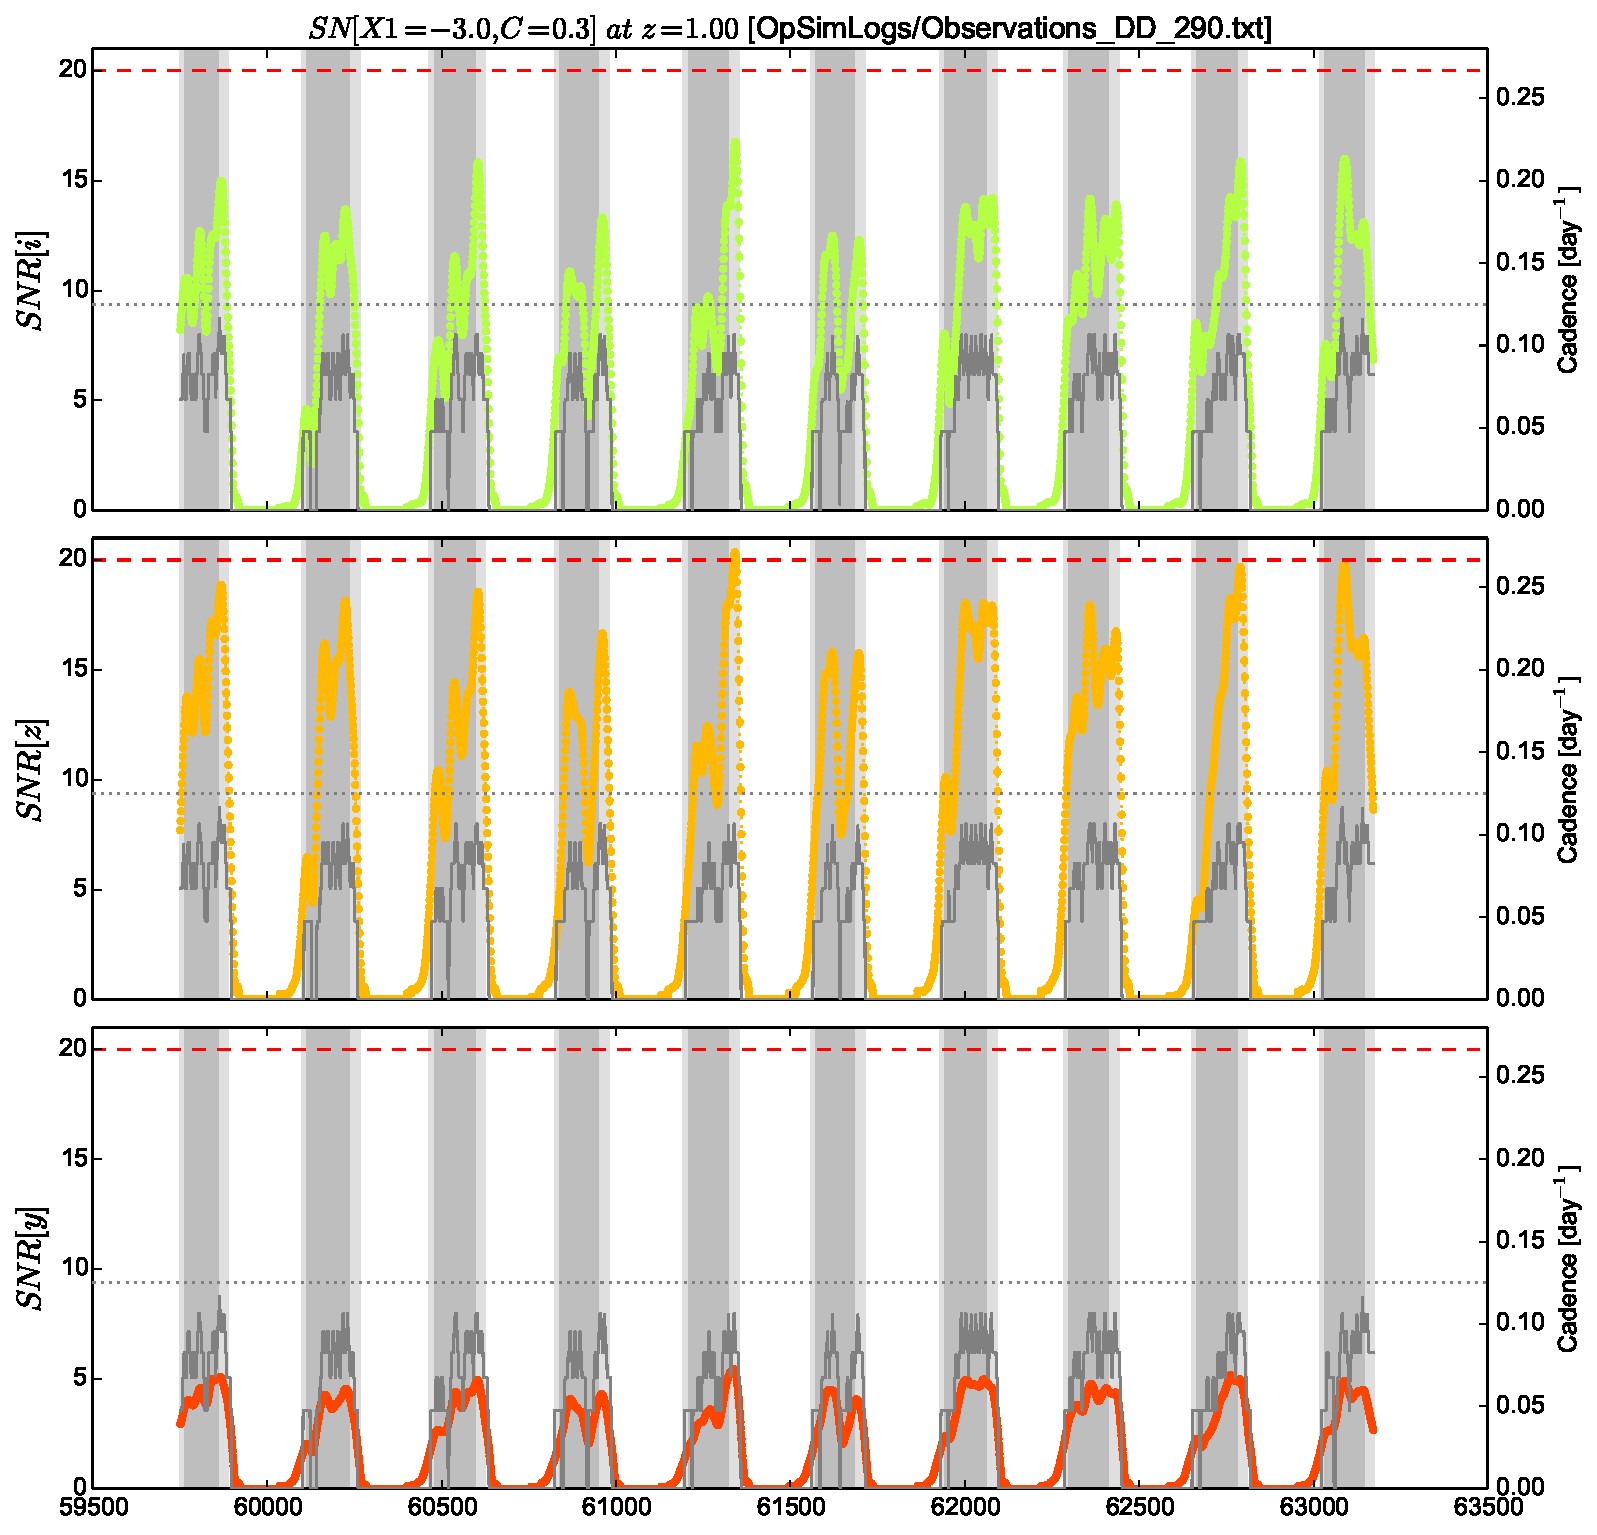
\includegraphics[width=\linewidth]{metric_DD_290.pdf}
    \caption{}
  \end{center}
\end{figure*}




% ----------------------------------------------------------------------
\section{The Wide LSST SN survey}
\subsection{The cadence from \code{Minion\_1016}}
\label{sec:results}

\begin{figure*}
\begin{center}
\subfigure[$g$]{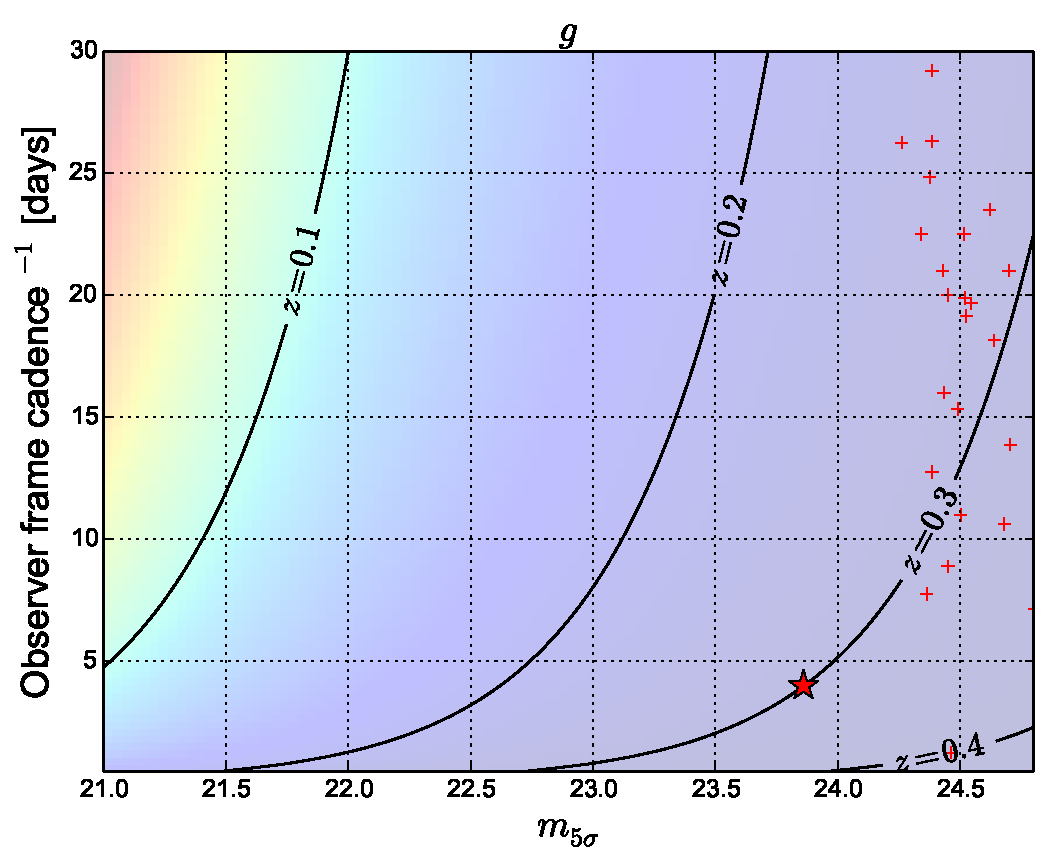
\includegraphics[width=0.48\linewidth]{m5_cadence_limits_wide_g.pdf}}
\subfigure[$r$]{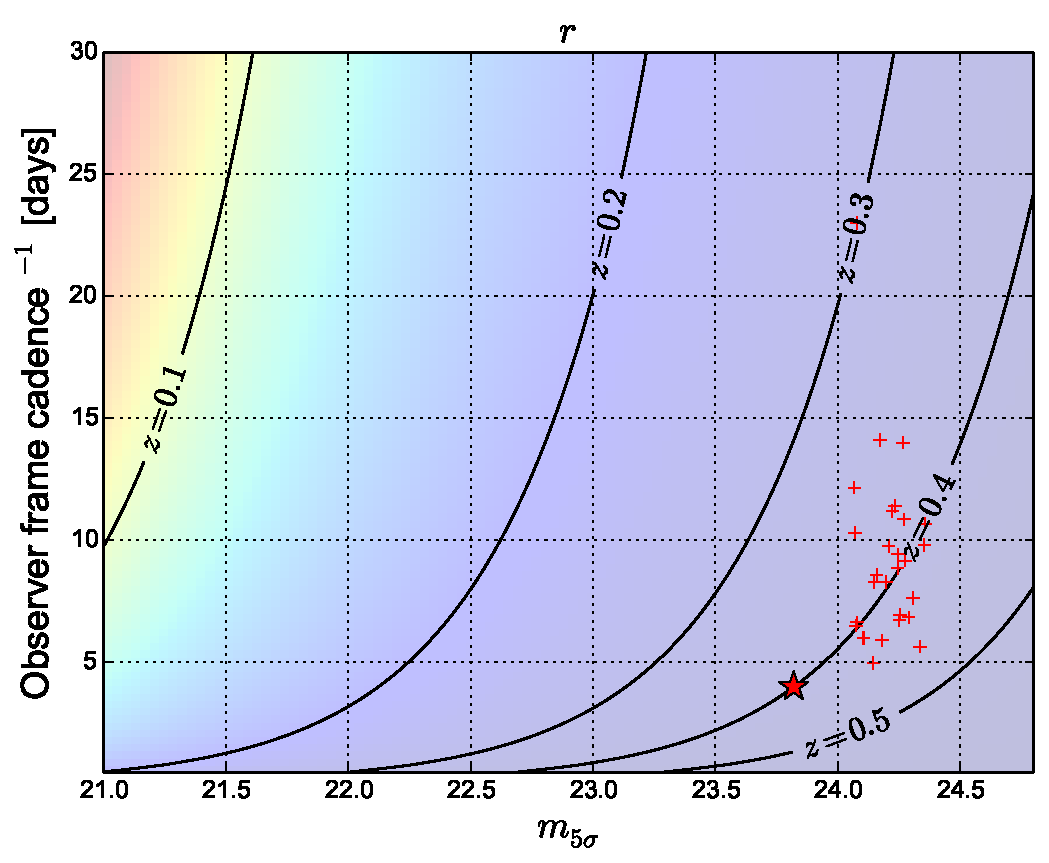
\includegraphics[width=0.48\linewidth]{m5_cadence_limits_wide_r.pdf}}\\
\subfigure[$i$]{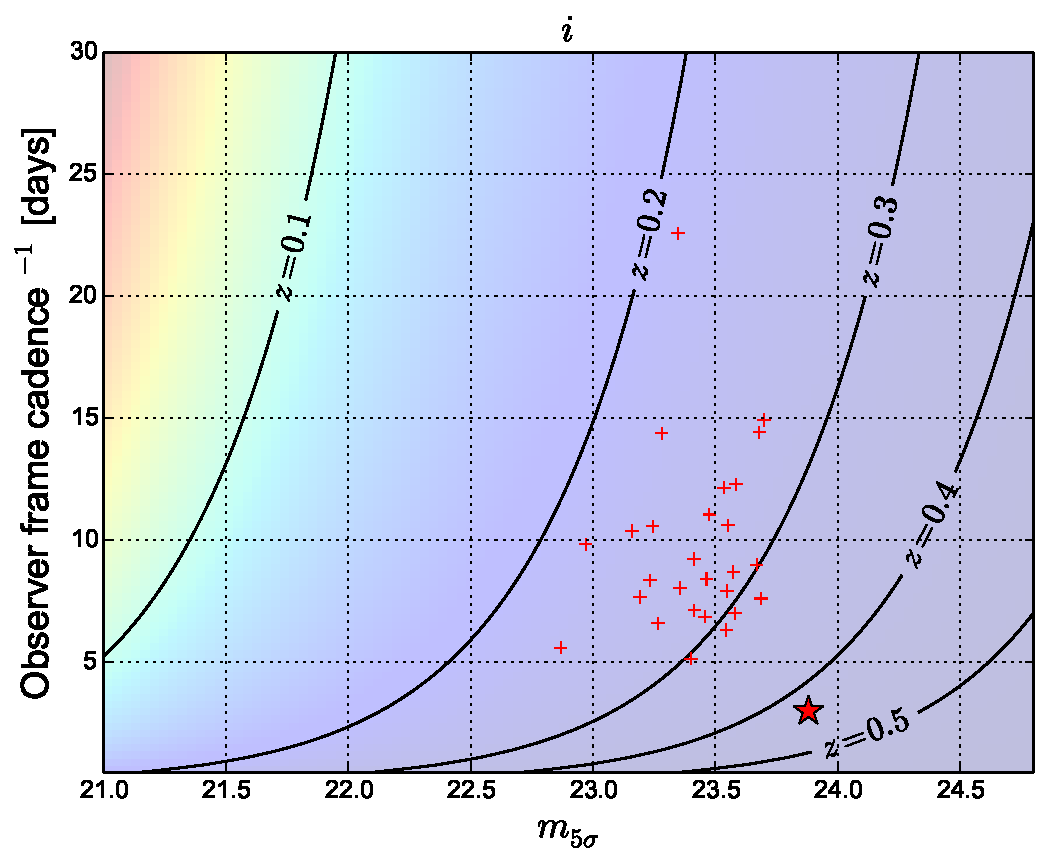
\includegraphics[width=0.48\linewidth]{m5_cadence_limits_wide_i.pdf}}
\subfigure[$z$]{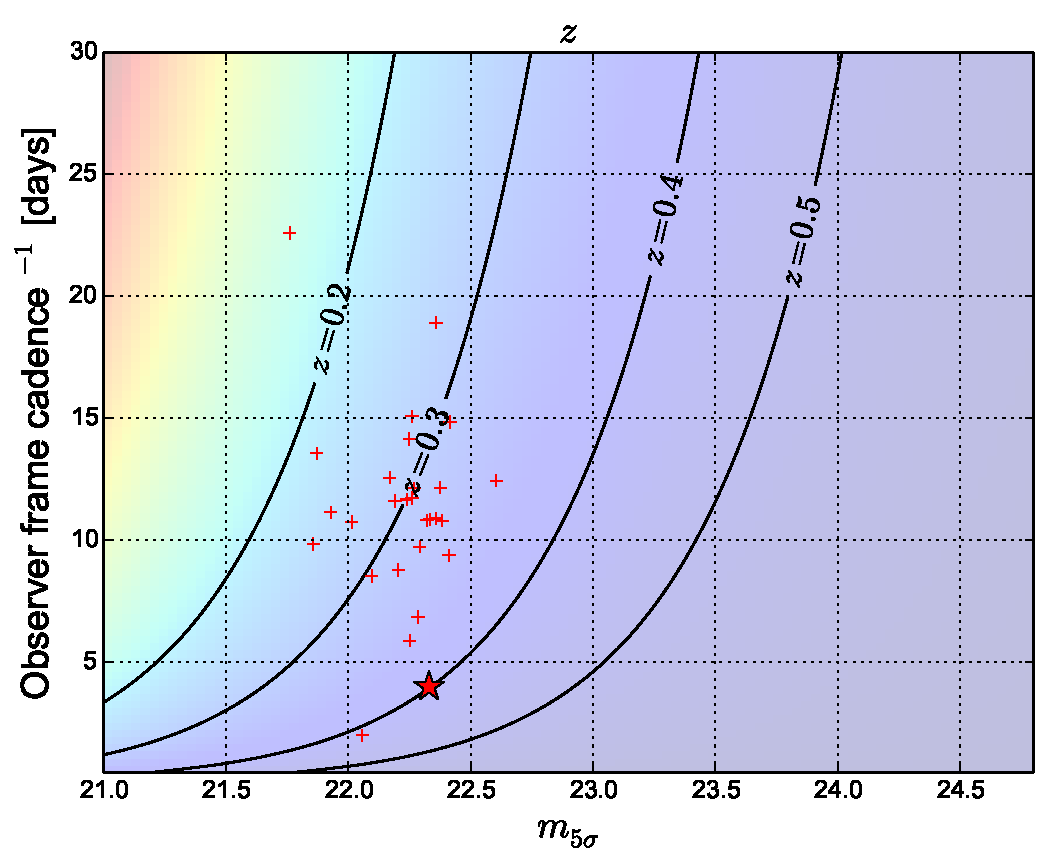
\includegraphics[width=0.48\linewidth]{m5_cadence_limits_wide_z.pdf}}
\caption{The cadence {\em vs.} depth requirements for the Wide survey,
  in the $g, r, i$ and $z$-bands. The color scale corresponds to the
  metric described in equation \ref{eqn:global_metric}.  The lines are
  the contour-levels computed for the limits indicated on table
  \ref{tab:cadence_depth_limit}. To fulfill the SNR requirements at a
  given redshift, one has to be {\em below} the corresponding
  line. The stars indicate an ambitious -- but attainable -- goal for
  a DDF survey.  The red crosses show what the survey can currently
  deliver according to \code{Minion\_1016}.}
\label{fig:m5_cadence_limits_wide}
\end{center}
\end{figure*}

\begin{figure*}[t]
  \begin{center}
    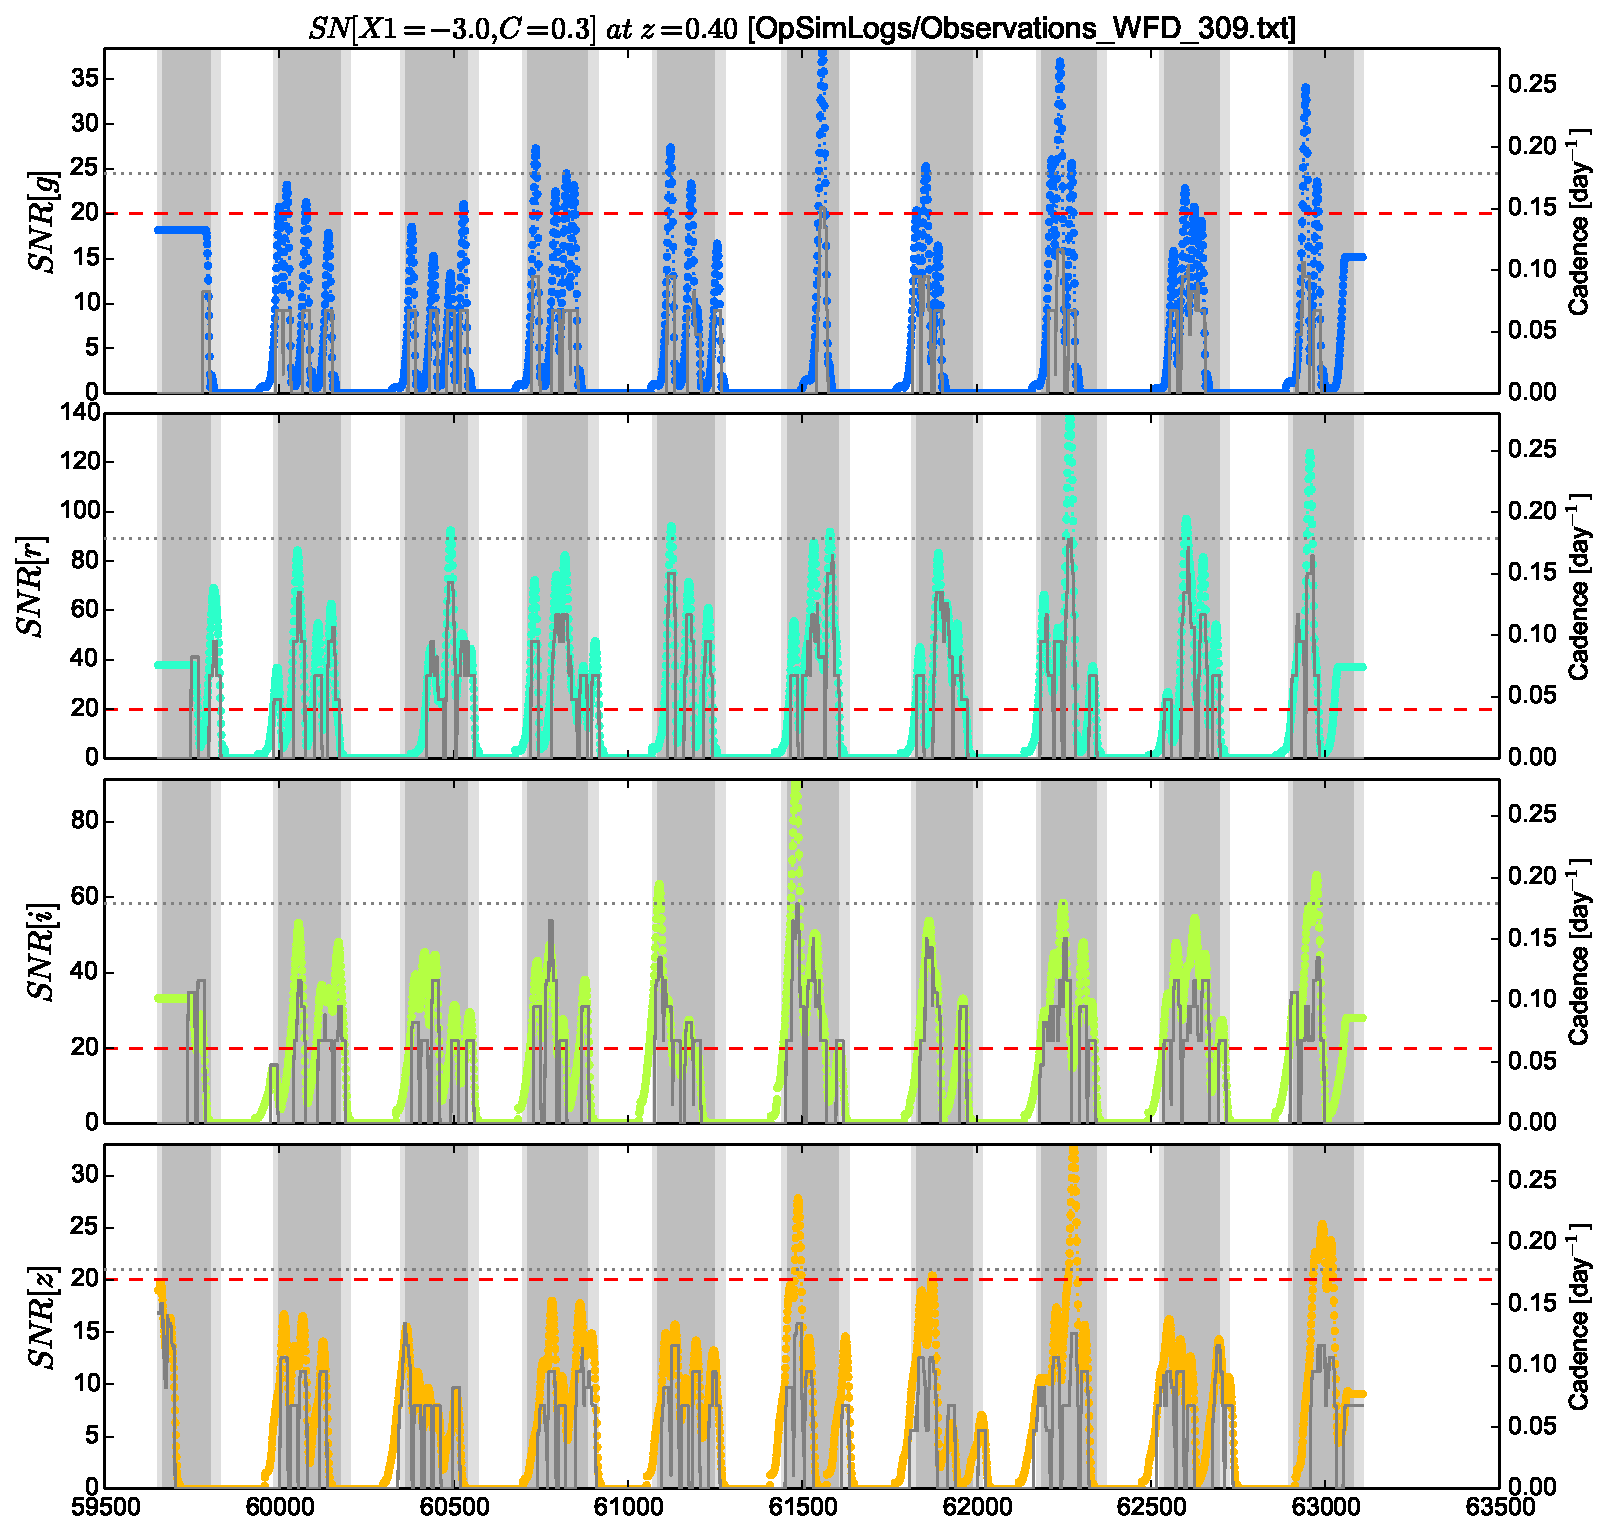
\includegraphics[width=\linewidth]{metric_WFD_309.pdf}
    \caption{}
  \end{center}
\end{figure*}



% \figref{example} shows an example figure, referred to with the \verb=\figref= command and the \code{fig:} prefix.
% \begin{figure}
% 
\includegraphics[width=0.9\columnwidth]{example.png}
% \caption{An example figure: the LSST DESC logo, copied from \code{texmf/logos/desc-logo.png} into \code{figures/example.png}. \label{fig:example}}
% \end{figure}

\subsection{The rolling cadence from \code{Minion\_1016}}
\label{sec:results}

% ----------------------------------------------------------------------

\section{The Rolling Cadence }
\label{sec:results}

% \figref{example} shows an example figure, referred to with the \verb=\figref= command and the \code{fig:} prefix.

% \begin{figure}
% 
\includegraphics[width=0.9\columnwidth]{example.png}
% \caption{An example figure: the LSST DESC logo, copied from \code{texmf/logos/desc-logo.png} into \code{figures/example.png}. \label{fig:example}}
% \end{figure}




% ----------------------------------------------------------------------

\section{Discussion}
\label{sec:discussion}

If you are planning on committing your paper to GitHub, it's a good idea to write your tex as one sentence per line.
This allows for an easier \code{diff} of changes.
It also makes sense to think of latex as \emph{code}, and sentences as logical statements, occupying one line each.
Each line must ``compile'' in the mind of the reader.


% ----------------------------------------------------------------------

\section{Conclusions}
\label{sec:conclusions}

We have presented design guidelines for the wide and deep LSST SN
surveys and discussed requirements on the survey depth and cadence.
We have developed a lightweight metric to assess whether a given
cadence matches these requirements without having to resort to an
extensive simulation.

We have evaluated the \code{Minion\_1016} cadence, on a series of DDF
and wide fields. We summarize our conclusions below:

\begin{itemize}
\item on the DDF fields, the survey is complete up to $z \sim
  0.65$. This is comparable to what was obtained with SNLS in the
  2000's but well below what should be an ambitious goal for LSST
  (produce a redshift limited SN~Ia Hubble diagram up to $z_{lim} \sim
  1$).

\item on the DDF fields, increasing the duration of the search seasons
  from 4.5 months to 6 months would allow to gain tremendously in
  statistics (almost a factor 2) at high redshift.
  
\item on the Wide fields, the redshift limit is of about $z \sim
  0.3$. A more ambitious target is rather $z_{lim} \sim 0.4$.  In the
  $g$-band, the regularity of the cadence should be improved.

\item we have shown that, by tweaking the cadence, one can reach a
  $z_{lim}$ of 0.9 for the DDF fields and $z_{lim} \sim 0.4$ on the
  Wide, in the same observing time budget.

\item it remains to be proven that these cadences can be reached
  within the constraints of the survey operations, as they are
  implemented in {\tt OpSim}.  We suggest implementing, in the OpSim
  scheduler, a dynamic scheduling algorithm based on the metrics
  discussed above.  
  
  To give orders of magnitudes, a reasonable target is a cadence of 4
  restframe days at the median redshift of the wide and deep surveys.
  This corresponds to an observer frame cadence of $\sim 5.2$ (resp
  6.8) days on the wide and the DDF respectively.

\item finally, the results presented here should be taken with a bit
  of caution.  As we discuss in appendix
  \ref{sec:lsst_instrument_models}, and shown on figure
  \ref{fig:lsst_model_summary}, the assessment of the instrument
  throughput and of the average observing conditions have been
  recently revised, and this revision has a very significant impact on
  the expected survey depth (almost half a magnitude per standard
  visit).  

  Furthermore, the average observing conditions used in
  \code{Minion\_{1016}} seem to be quite pessimistic.  In particular,
  the \code{Minion\_{1016}} sky brightness is probably too bright,
  especially in the $y$-band.
\end{itemize}

The results presented in this note will be updated as revised OpSim
cadences become available.


% ----------------------------------------------------------------------

\subsection*{Acknowledgments}

Here is where you should add your specific acknowledgments, remembering that some standard thanks will be added via the \code{acknowledgments.tex} and \code{contributions.tex} files.

% 
This is the text imported from \code{acknowledgments.tex}, and will be replaced by some standard LSST DESC boilerplate at some point.
% 


\input{contributions}

%{\it Facilities:} \facility{LSST}

% Include both collaboration papers and external citations:
\bibliography{lsstdesc,main}





\appendix

\section{LSST instrument models}
\label{sec:lsst_instrument_models}

To prepare this study, we have used two instrument models.  One is
based on the numbers reported in \cite[][LSE-40 hereafter]{LSE-40}.
We report the main ingredients of this model in table \ref{tab:lse40}. 

The other model is described in \cite[][hereafter
SMTN-002)]{SMTN-002}, which constitutes a preliminary update of
LSE-40.  The current version OpSim relies on SMTN-002. An we therefore
adopt this model as our reference. Key quantities of SMTN-002 are
listed in table \ref{tab:smtn002}.

We note that both models differ very significantly. In particular (1)
the throughput of SMTN-002 is almost 50\% lower.


\begin{table}
\begin{center}
\caption{LSE-40 model}
\label{tab:lse40}
\begin{tabular}{l|cccccc}
\hline 
\hline 
\multicolumn{7}{c}{{\bf General}} \\
\hline
Pixel size & \multicolumn{6}{r}{0.2 arcsec} \\
RO noise   & \multicolumn{6}{r}{9 $e^-$}    \\
\hline
\multicolumn{7}{c}{{\bf Zero Points @ X=1 [AB, fluxes in e$^-$/s]}} \\
\hline
           &  $u$ & $g$ & $r$ & $i$ & $z$ & $y$ \\
LSE-40     & 27.09 & 28.58 & 28.50 & 28.34 & 27.95 & 27.18 \\
snsim      & 27.05 & 28.59 & 28.53 & 28.38 & 27.99 & 27.22 \\
\hline
\multicolumn{7}{c}{{\bf median seeing [arcsec]}} \\
\hline
LSE-40 / snsim  &  0.77 &  0.73 &  0.70 &  0.67 &  0.65 &  0.63 \\
\hline
\multicolumn{7}{c}{{\bf Dark sky [AB mag / arcsec$^2$]}}   \\
\hline
LSE-40     & 22.92 & 22.27 & 21.20 & 20.47 & 19.59 & 18.63 \\
snsim      & 22.95 & 22.26 & 21.20 & 20.47 & 19.60 & 18.61 \\
\hline
\multicolumn{7}{c}{{\bf NEA [pixel$^2$]}}   \\
\hline
snsim (Moffat, $\beta=4.5$)     & 41.5  & 37.4  & 34.5  & 31.7 & 29.9  & 28.6  \\
\hline
\multicolumn{7}{c}{{\bf Limiting mag ($5 \sigma$), 30-s visit}}   \\
\hline
LSE-40                        & 24.22  &  25.15 &  24.74  &  24.38  &  23.80  &  22.93  \\
snsim (Moffat, $\beta=7$)     & 24.27  &  25.18 &  24.73  &  24.36  &  23.77  &  22.92  \\
\hline
\end{tabular}
\end{center}
\end{table}


\begin{table}
\begin{center}
\caption{SMTN-002 model}
\label{tab:smtn002}
\begin{tabular}{l|cccccc}
\hline 
\hline 
\multicolumn{7}{c}{{\bf General}} \\
\hline
Pixel size & \multicolumn{6}{r}{0.2 arcsec} \\
RO noise   & \multicolumn{6}{r}{9 $e^-$}    \\
\hline
\multicolumn{7}{c}{{\bf Zero Points @ X=1 [AB, fluxes in e$^-$/s]}} \\
\hline
           &  $u$ & $g$ & $r$ & $i$ & $z$ & $y$ \\
SMTN-002   & 26.50 & 28.30 & 28.13 & 27.79 & 27.40 & 26.58 \\
snsim      & 26.48 & 28.34 & 28.17 & 27.85 & 27.46 & 26.63 \\
\hline
\multicolumn{7}{c}{{\bf median seeing [arcsec]}} \\
\hline
SMTN-002 / snsim  &  0.92 &  0.87 &  0.83 &  0.80 &  0.78 &  0.76 \\
\hline
\multicolumn{7}{c}{{\bf Dark sky [AB mag / arcsec$^2$]}}   \\
\hline
SMTN-002   & 22.95 & 22.24 & 21.20 & 20.47 & 19.60 & 18.63 \\ %% line 1 of Table 2
snsim      & 22.98 & 22.23 & 21.19 & 20.46 & 19.60 & 18.61 \\
\hline
\multicolumn{7}{c}{{\bf NEA [pixel$^2$]}}   \\
\hline
snsim (Moffat, $\beta=7$)     & 58.8  & 52.7  & 48.0  & 44.7  & 42.6  & 40.5  \\
\hline
\multicolumn{7}{c}{{\bf Limiting mag ($5 \sigma$), 30-s visit}}   \\
\hline
SMTN-002                    &  23.60     &  24.83     &  24.38     &   23.92    &  23.35     &  22.44  \\
snsim (Moffat, $\beta=7$)   &  23.61     &  24.83     &  24.35     &   23.88    &  23.30     &  22.43  \\
\hline
\end{tabular}
\end{center}
\end{table}


\begin{figure}[t]
\begin{center}
\subfigure[LSE-40]{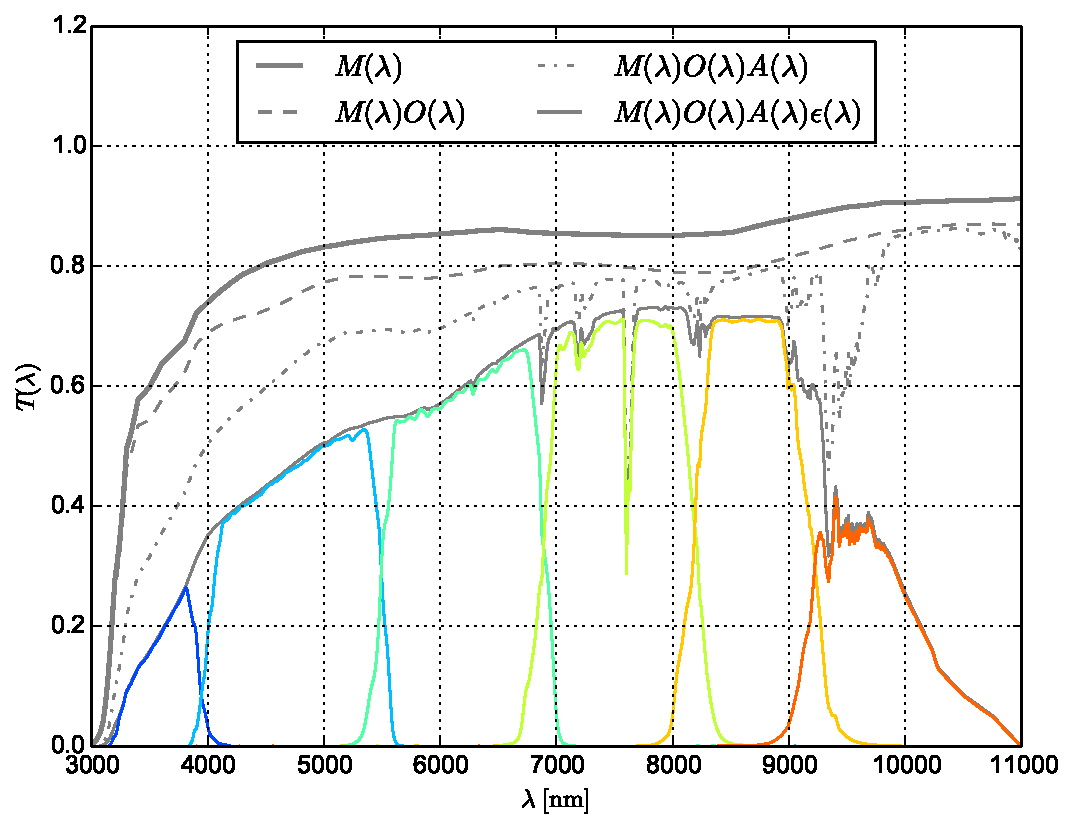
\includegraphics[width=0.45\linewidth]{lse_40_passbands.pdf}}
\subfigure[SMTN-002]{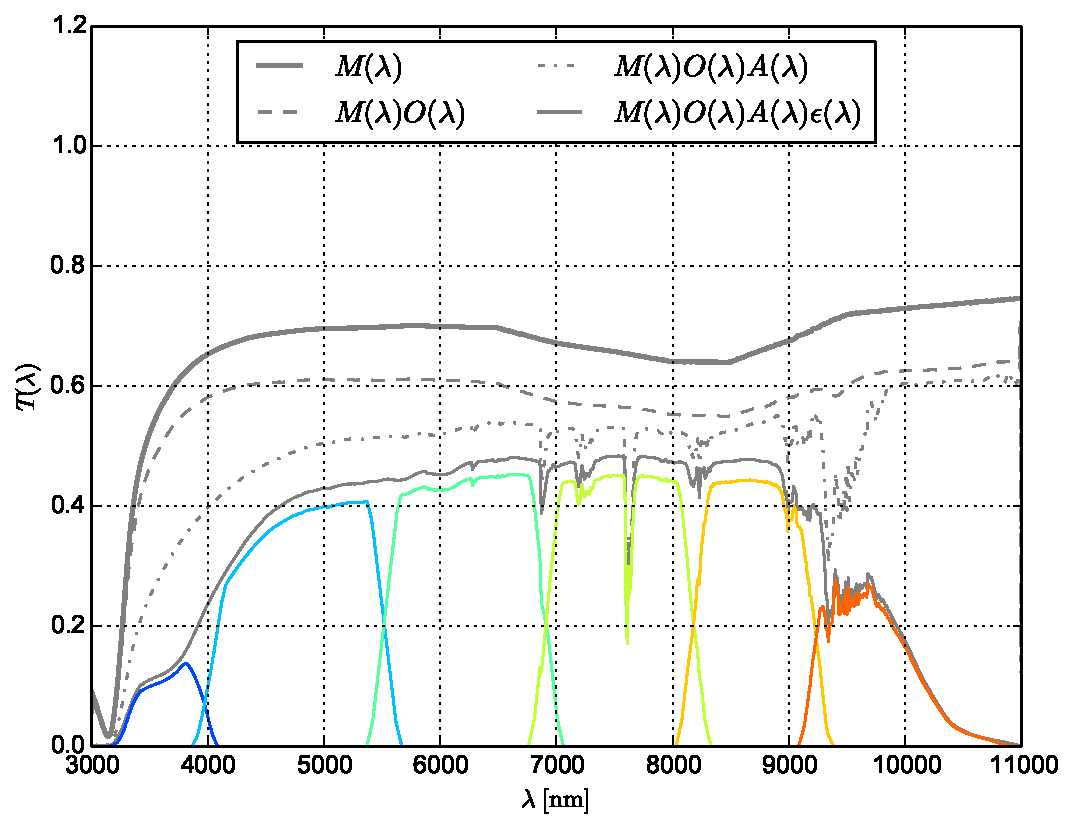
\includegraphics[width=0.45\linewidth]{smtn002_passbands.pdf}}
\caption{Instrument passbands}
\end{center}
\end{figure}


\begin{figure}[t]
\begin{center}
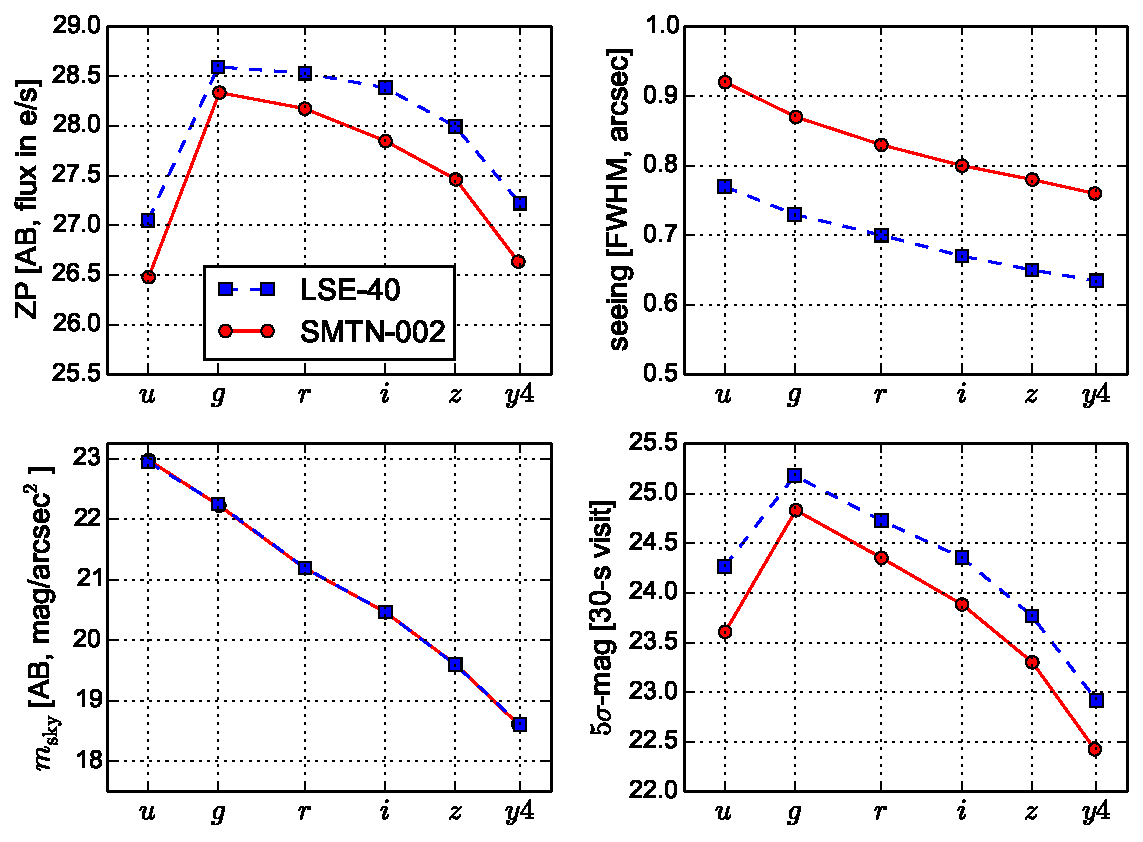
\includegraphics[width=\linewidth]{lsst_model_summary.pdf}
\caption{Zero-points, median seeing, dark sky mags and limiting mags}
\label{fig:lsst_model_summary}
\end{center}
\end{figure}


\section{Additional figures}

\begin{figure}[t]
  \begin{center}
    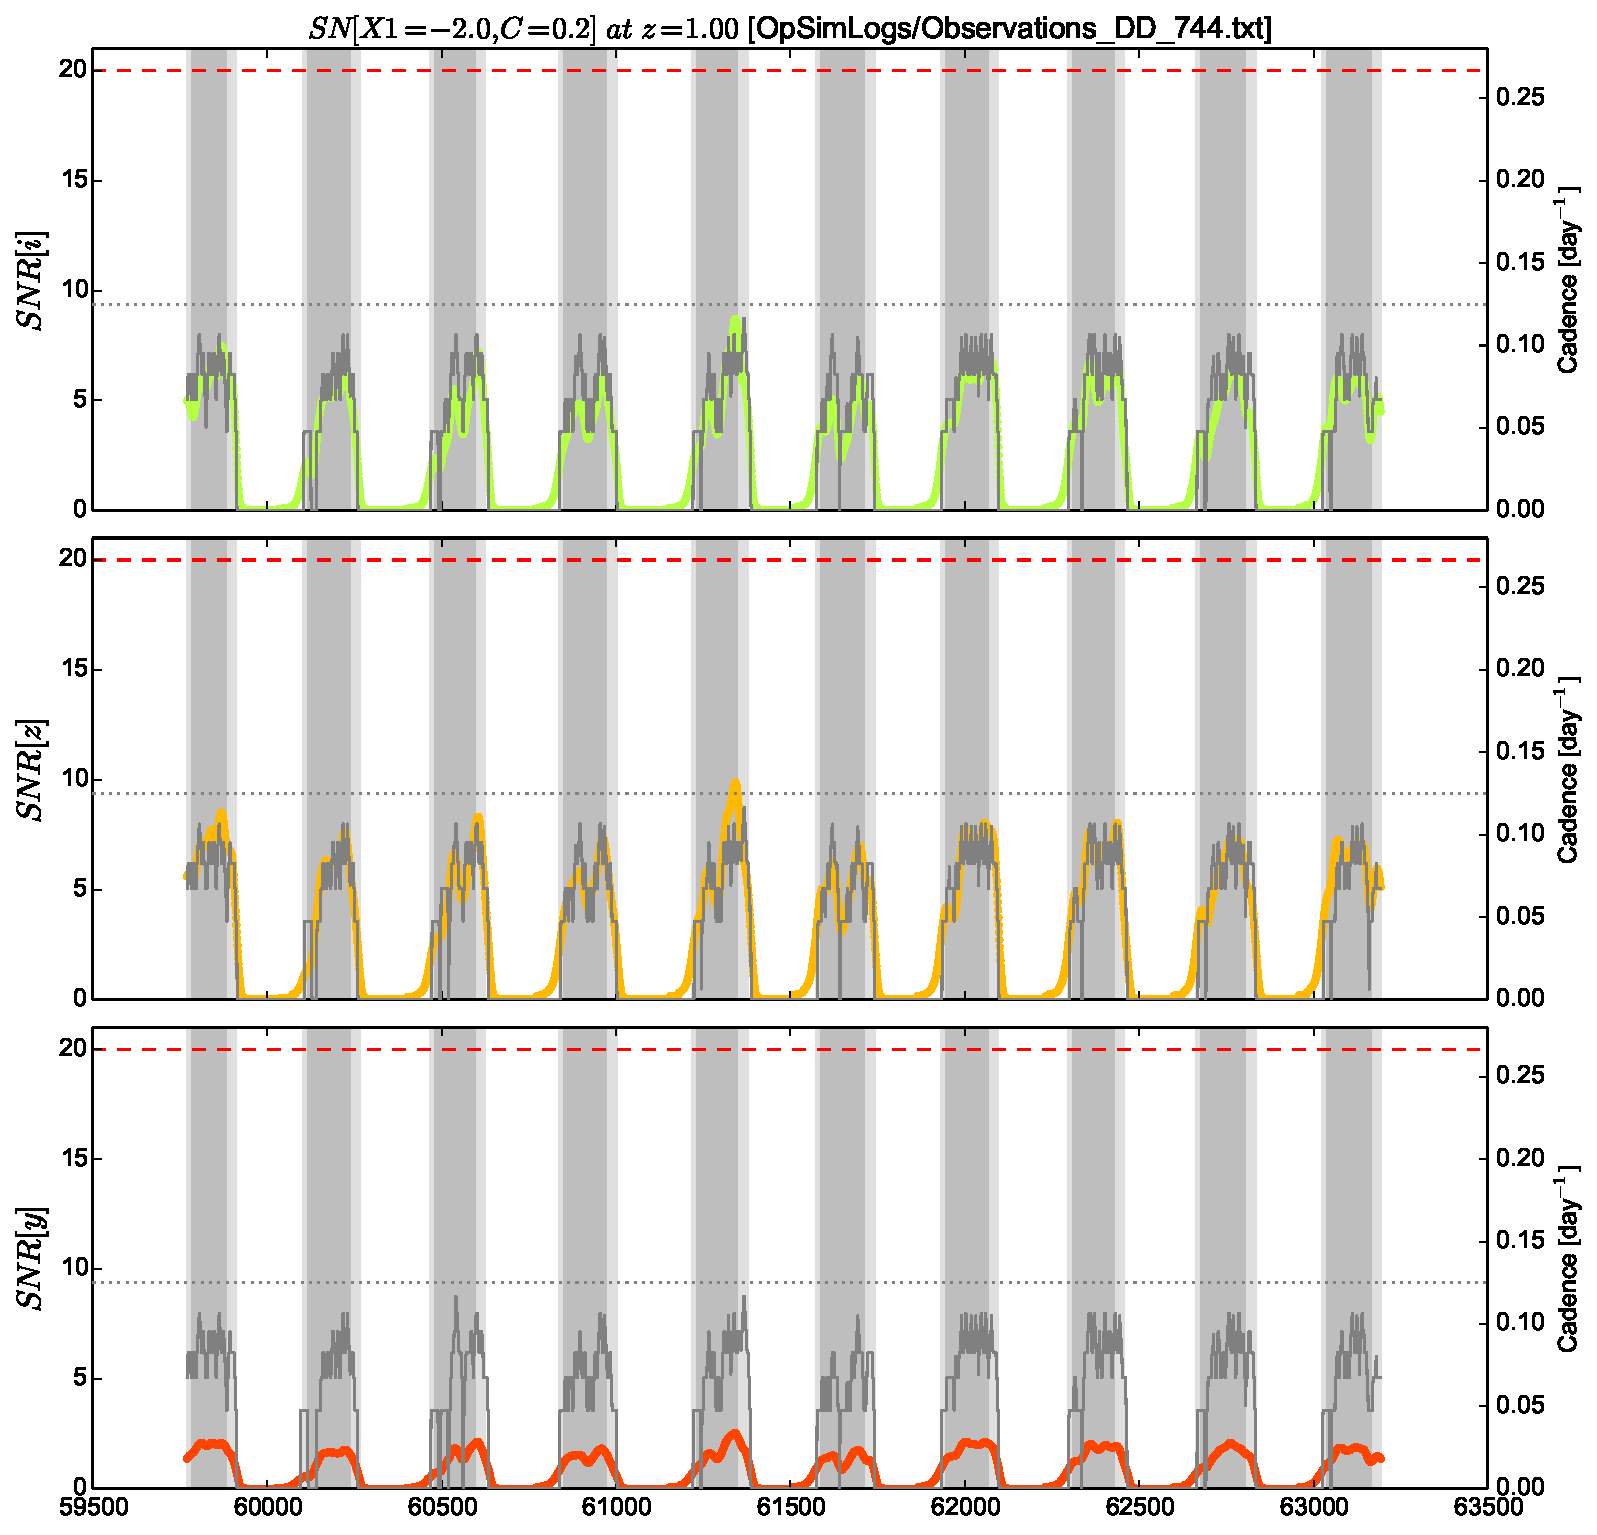
\includegraphics[width=\linewidth]{metric_DD_744.pdf}
    \caption{}
  \end{center}
\end{figure}


\begin{figure}[t]
  \begin{center}
    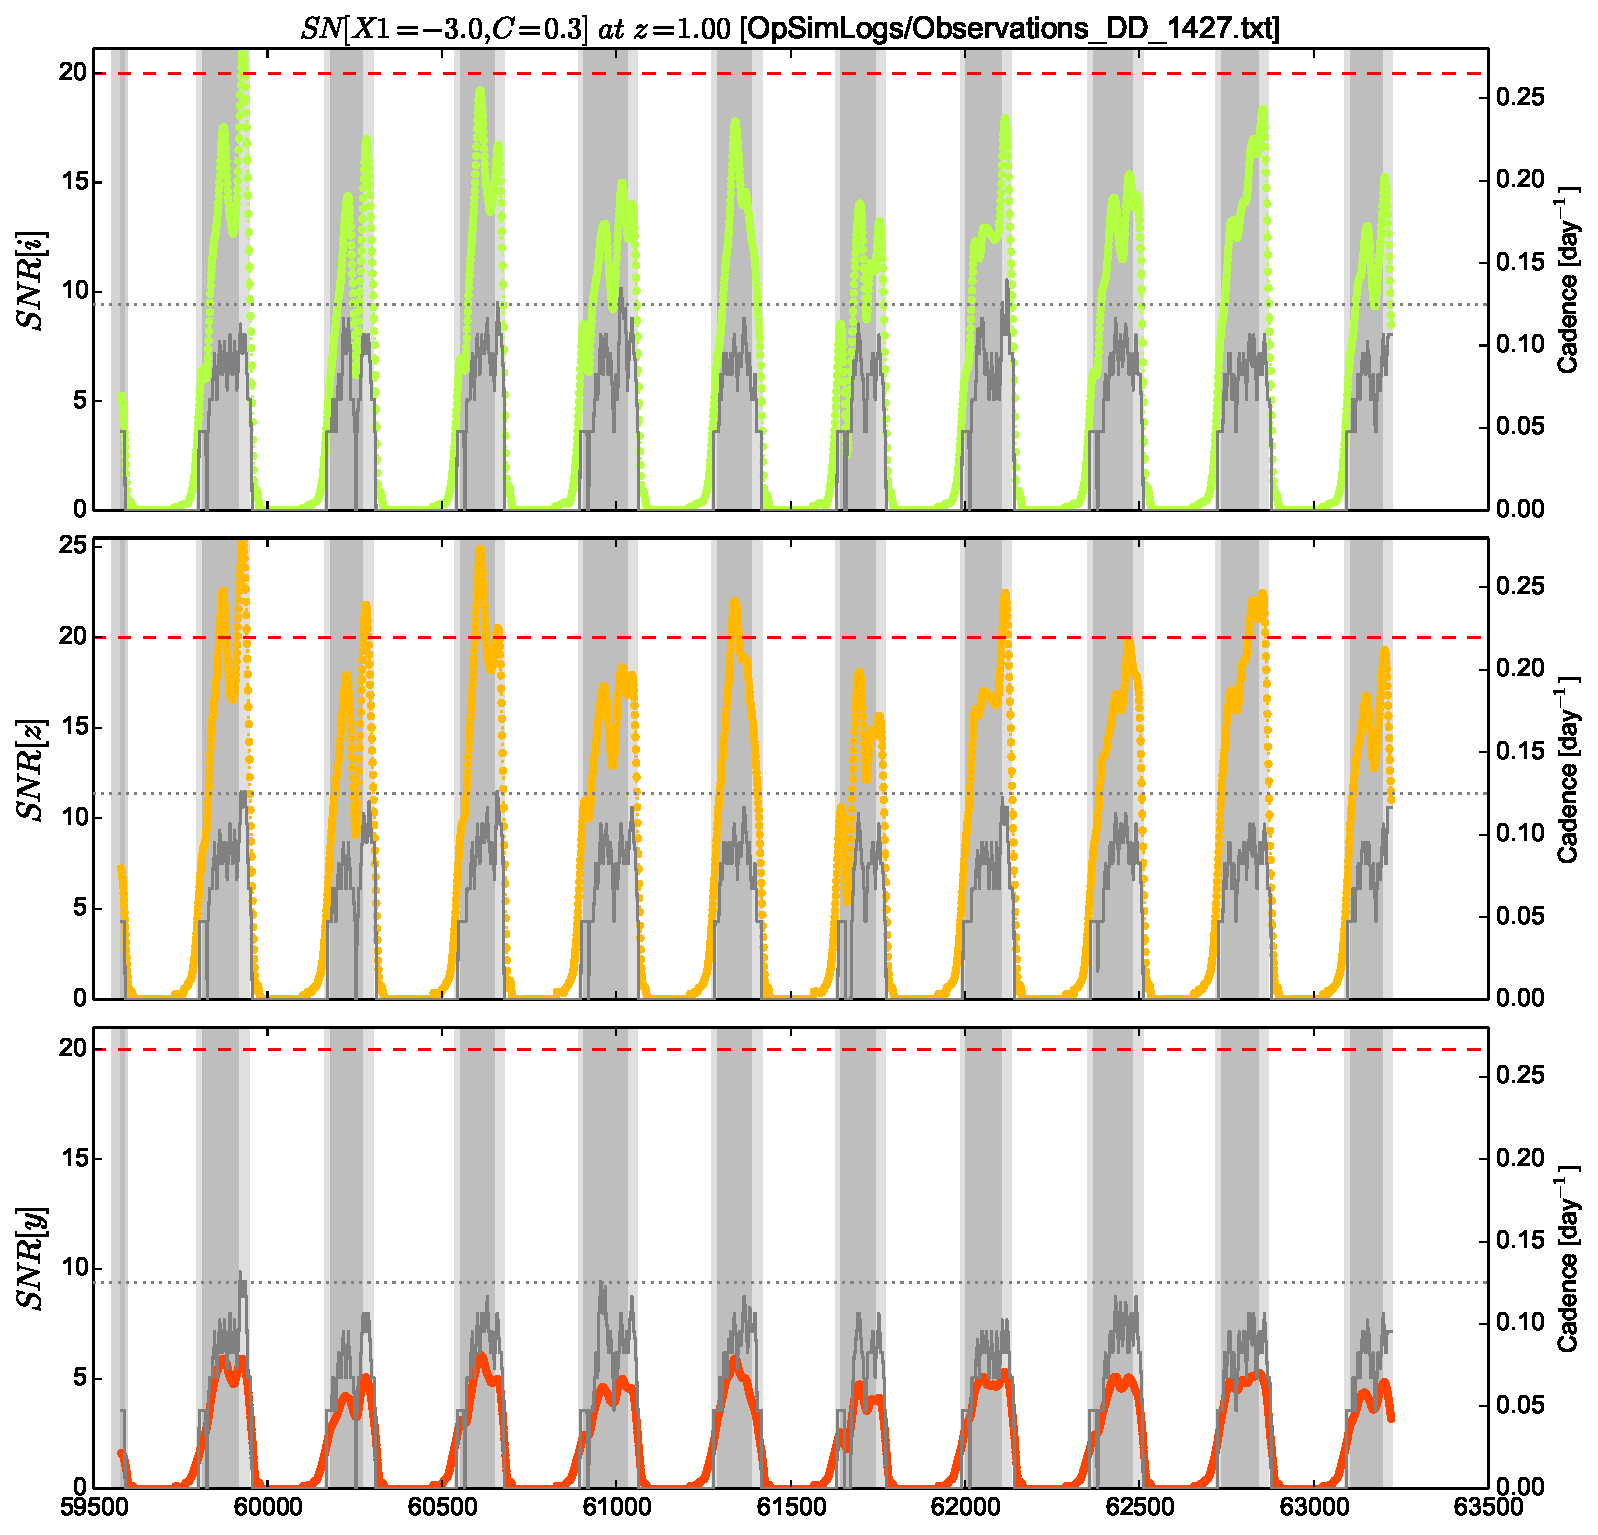
\includegraphics[width=\linewidth]{metric_DD_1427.pdf}
    \caption{}
  \end{center}
\end{figure}

\begin{figure}[t]
  \begin{center}
    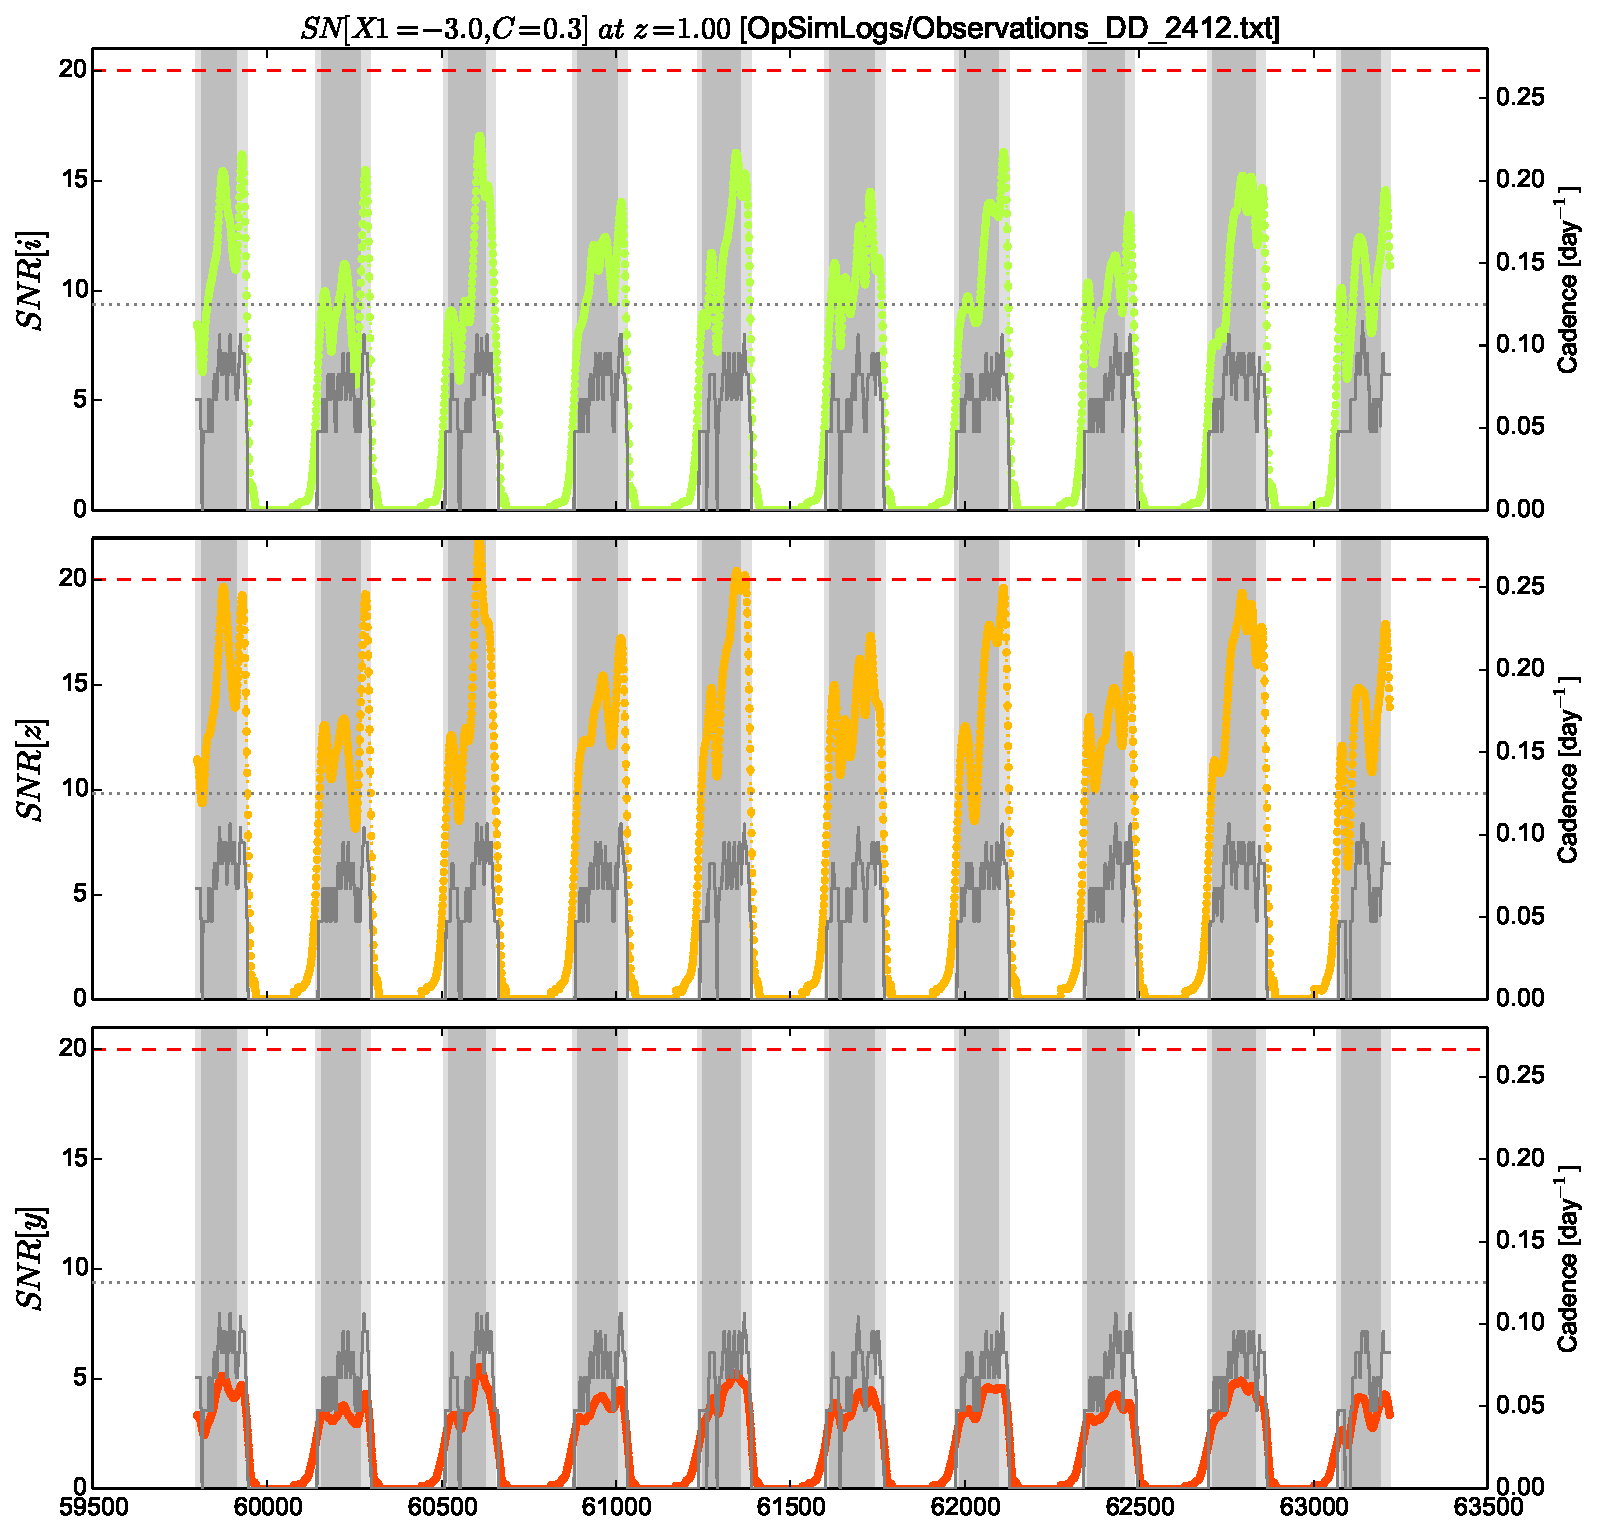
\includegraphics[width=\linewidth]{metric_DD_2412.pdf}
    \caption{}
  \end{center}
\end{figure}

\begin{figure}[t]
  \begin{center}
    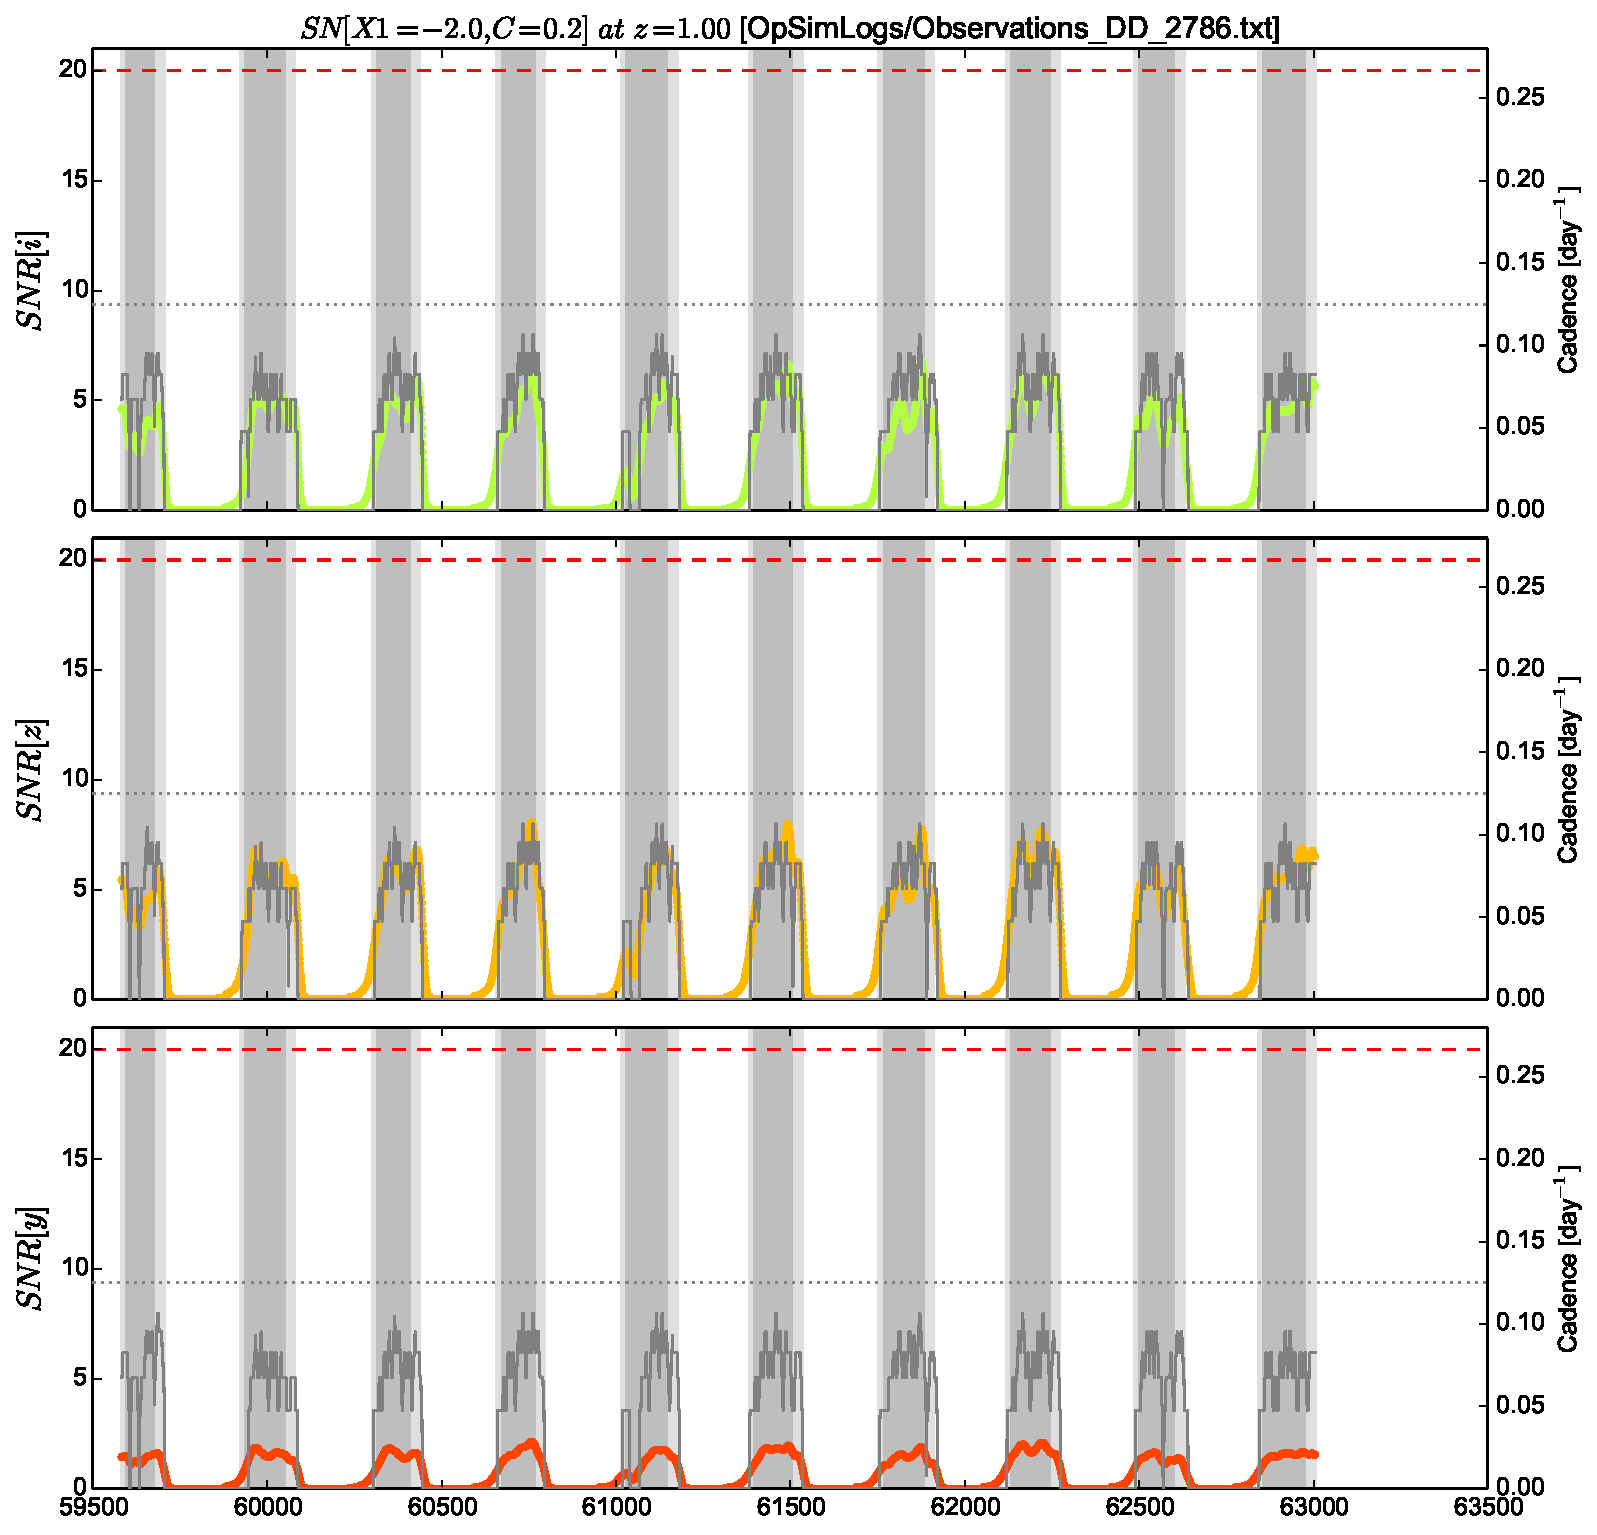
\includegraphics[width=\linewidth]{metric_DD_2786.pdf}
    \caption{}
  \end{center}
\end{figure}



\begin{figure*}[t]
  \begin{center}
    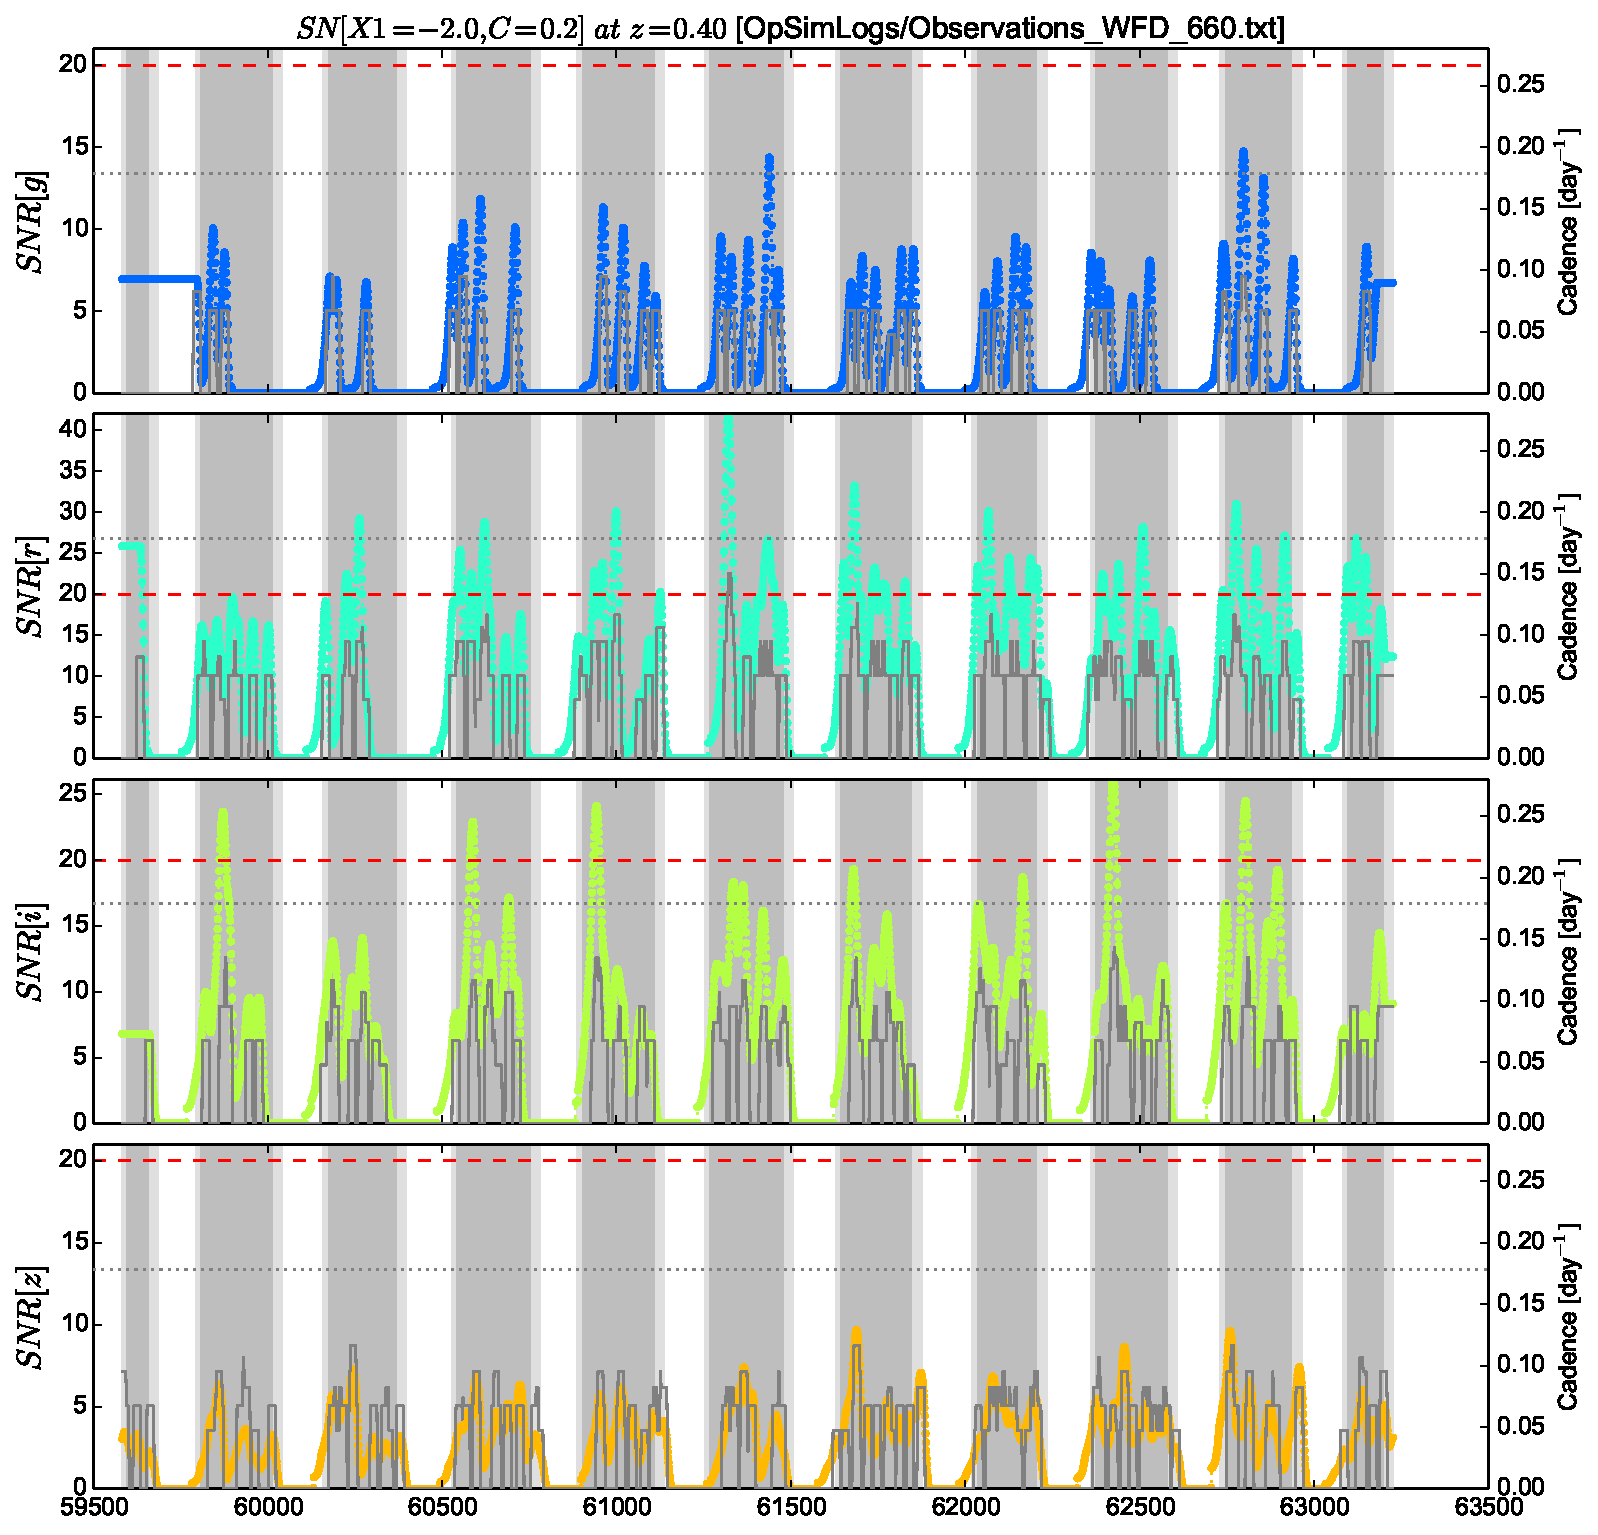
\includegraphics[width=\linewidth]{metric_WFD_660.pdf}
    \caption{}
  \end{center}
\end{figure*}

\begin{figure*}[t]
  \begin{center}
    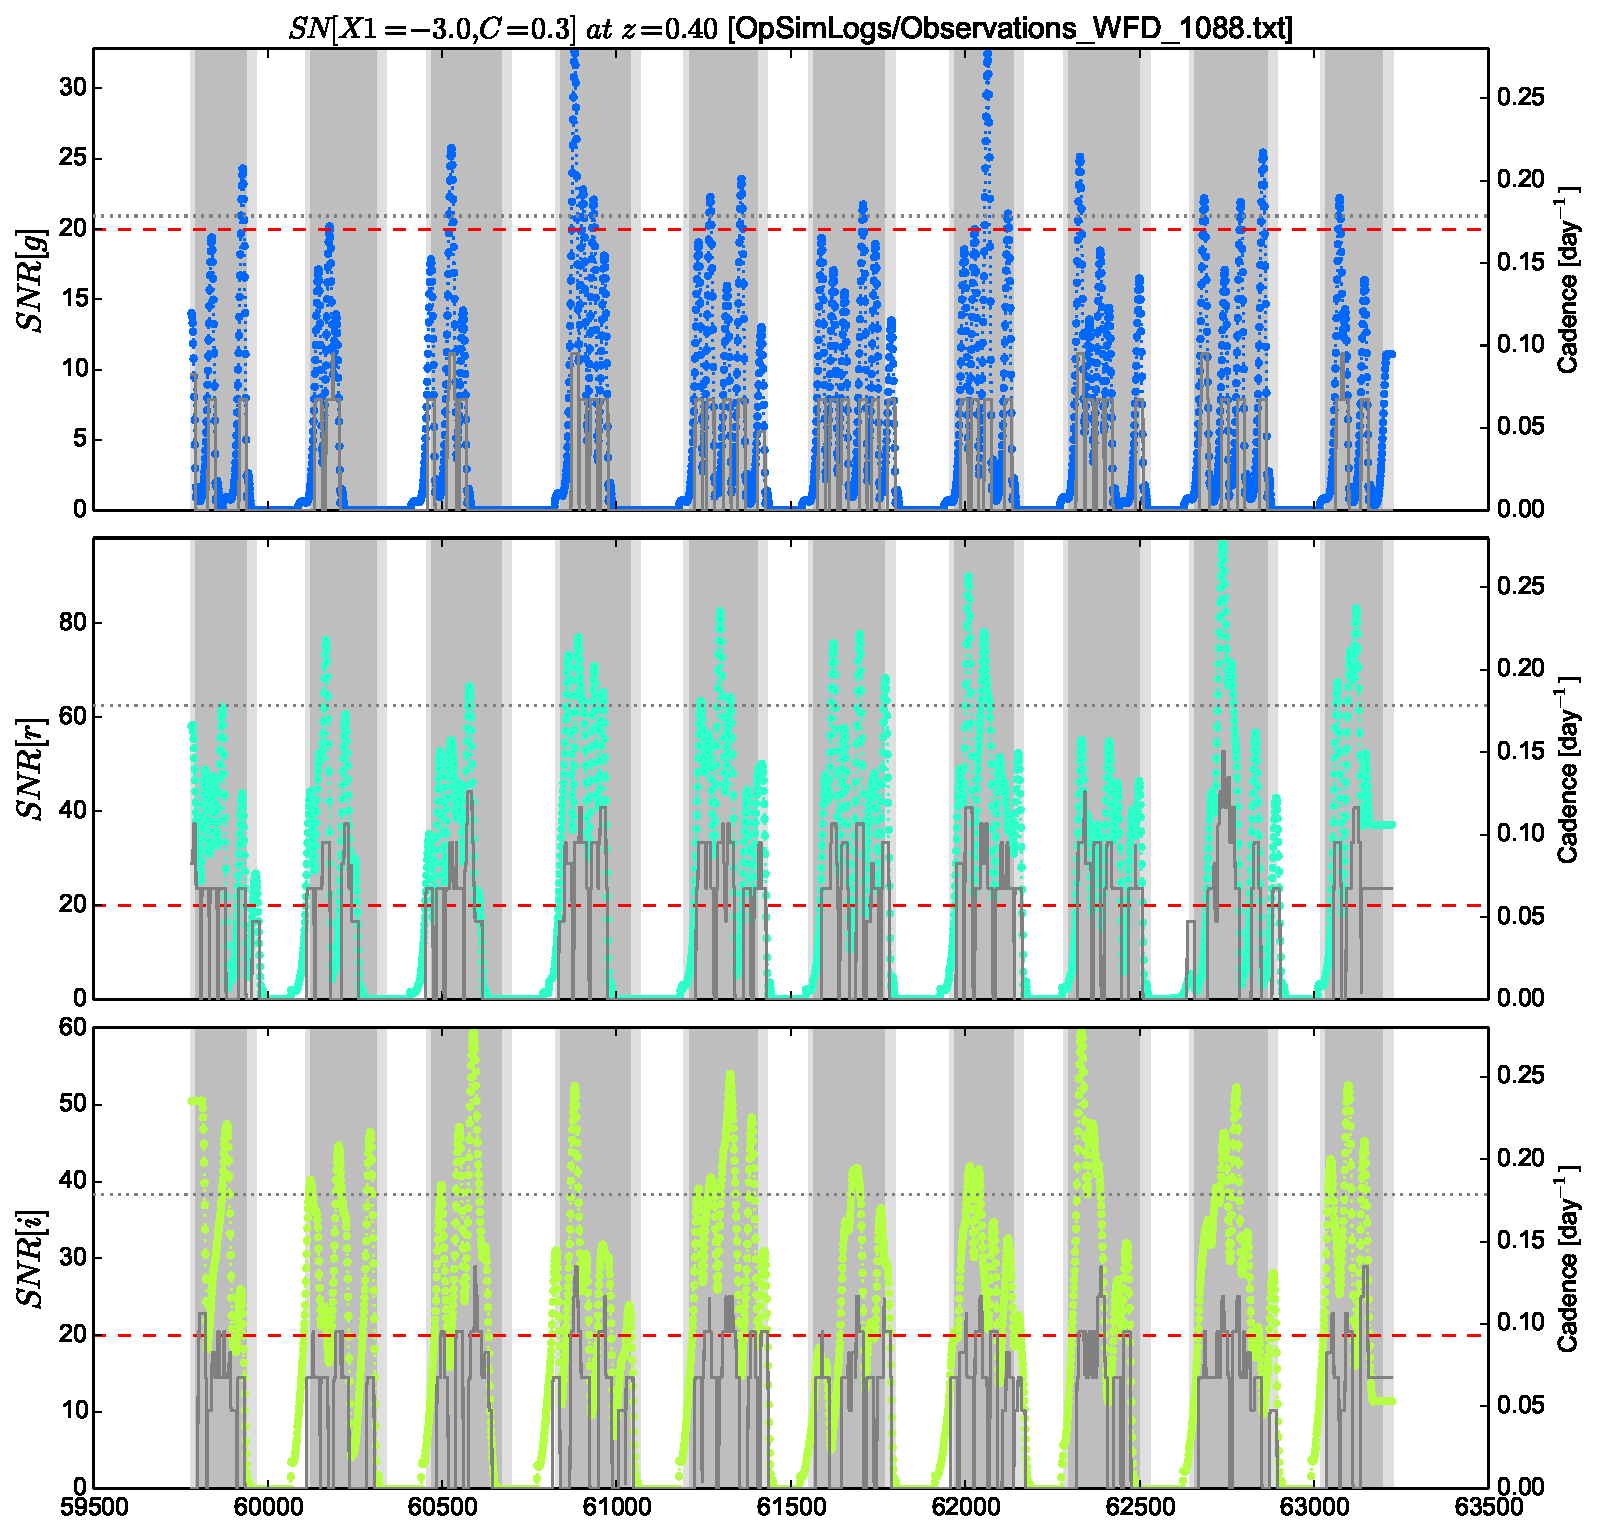
\includegraphics[width=\linewidth]{metric_WFD_1088.pdf}
    \caption{}
  \end{center}
\end{figure*}




\end{document}
% ======================================================================
% 








% There are a number of useful \LaTeX\xspace commands predefined in
% \code{macros.tex}.  Notice that the section labels are prefixed with
% \code{sec:} to allow the use of the \verb=\secref= command to
% reference a section (\ie, \secref{intro}).  Figures can be referenced
% with the \verb=\figref= command, which assumes that the figure label
% is prefixed with \code{fig:}.  In \figref{example} we show an example
% figure.  You'll notice that the actual figure file is found in the
% \code{figures} directory.  However, because we have specified this
% directory in our \verb=\graphicspath= we do not need to explicitly
% specify the path to the image.

% The \code{macros.tex} package also contains some conventional
% scientific units like \angstrom, \GeV, \Msun, etc. and some editorial
% tools for highlighting \FIXME{issues}, \CHECK{text to be checked},
% \COMMENT{comments}, and \NEW{new additions}.
